\chapter{Proposta}
    \label{chap:Proposta}

Neste capítulo, será retomada a \nameref{ContextualizaçãoProsposta}, para maior compreensão sobre o contexto no qual esse trabalho atua. Sendo assim, será apresentada a aplicação escolhida como foco de estudo. Em seguida, tem-se a \nameref{ProvaConceito}, conferindo informações sobre a aplicação \nameref{Shopee}, em sua versão atual. Há ainda menção à \nameref{AnaliseAttrakDiffR}, junto ao público alvo. Por fim, apresenta-se o \nameref{ResumoProposta}.


\section{Contextualização} 
    \label{ContextualizaçãoProsposta}

Este trabalho tem como objetivo o estudo sobre experiência de usuário no domínio de Comércio Eletrônico Móvel. Sendo assim, é necessária a identificação das principais dificuldades encontradas pelos usuários ao interagirem com plataformas de Comércio Eletrônico Móvel mais utilizadas no Brasil. Segundo \citeonline{FabricioUX}, de forma mais sucinta, a Usabilidade é um critério qualitativo focado em aspectos de \textit{design} de interfaces, apoiando-se em práticas que possibilitem que essas interfaces sejam mais facilmente utilizadas. Dentre as preocupações da Usabilidade, destacam-se: se o usuário consegue realizar uma tarefa sem transtorno ou demora em um número razoável de passos; se as informações são fáceis de entender, e se a experiência foi positiva, ou se o usuário saiu cognitivamente exausto. Já a Experiência do Usuário é um conceito ainda mais subjetivo. Procurando conferir uma visão mais objetiva e direta, projetar uma experiência do usuário pode ser algo desafiador, e que envolve identificar todos os aspectos da interação do usuário com o produto, o serviço ou ambiente em questão.

Segundo a pesquisa \citeonline{PesquisaMCommerce} sobre Pagamentos e Comércio pelo Celular no Brasil, considerando todos os dispositivos móveis disponíveis, os aplicativos de compras Shopee e Mercado Livre encontram-se liderando o \textit{ranking} de popularidade de comércio móvel no Brasil. Já para pesquisa \citeonline{ConversionDocs}, Figuras \ref{fig07} e \ref{aplim}, que considera apenas aplicações com sistema operacional Android, o Mercado Livre lidera o \textit{ranking} do comércio móvel.

\begin{figure}[ht]
    \centering
    \caption{\textit{Ranking} do Comércio Eletrônico Mais Utilizados em Android}
    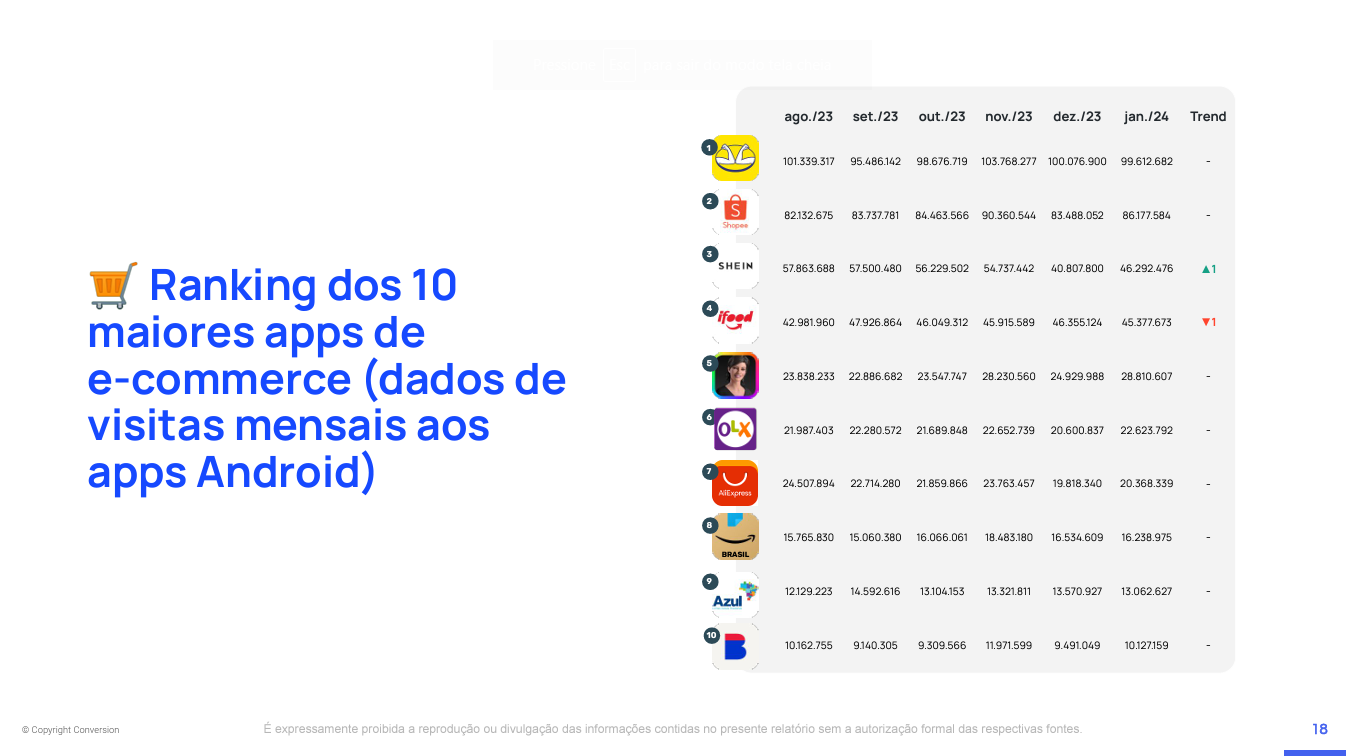
\includegraphics[keepaspectratio=true,scale=0.5]{figuras/cap05ConversionJan2024_3.png}
    \legend{Fonte: \cite{ConversionDocs}}
    \label{fig07}
\end{figure}

\begin{figure}[ht]
    \centering
    \caption{Aplicações de M-Commerce Mais Usados do Brasil}
    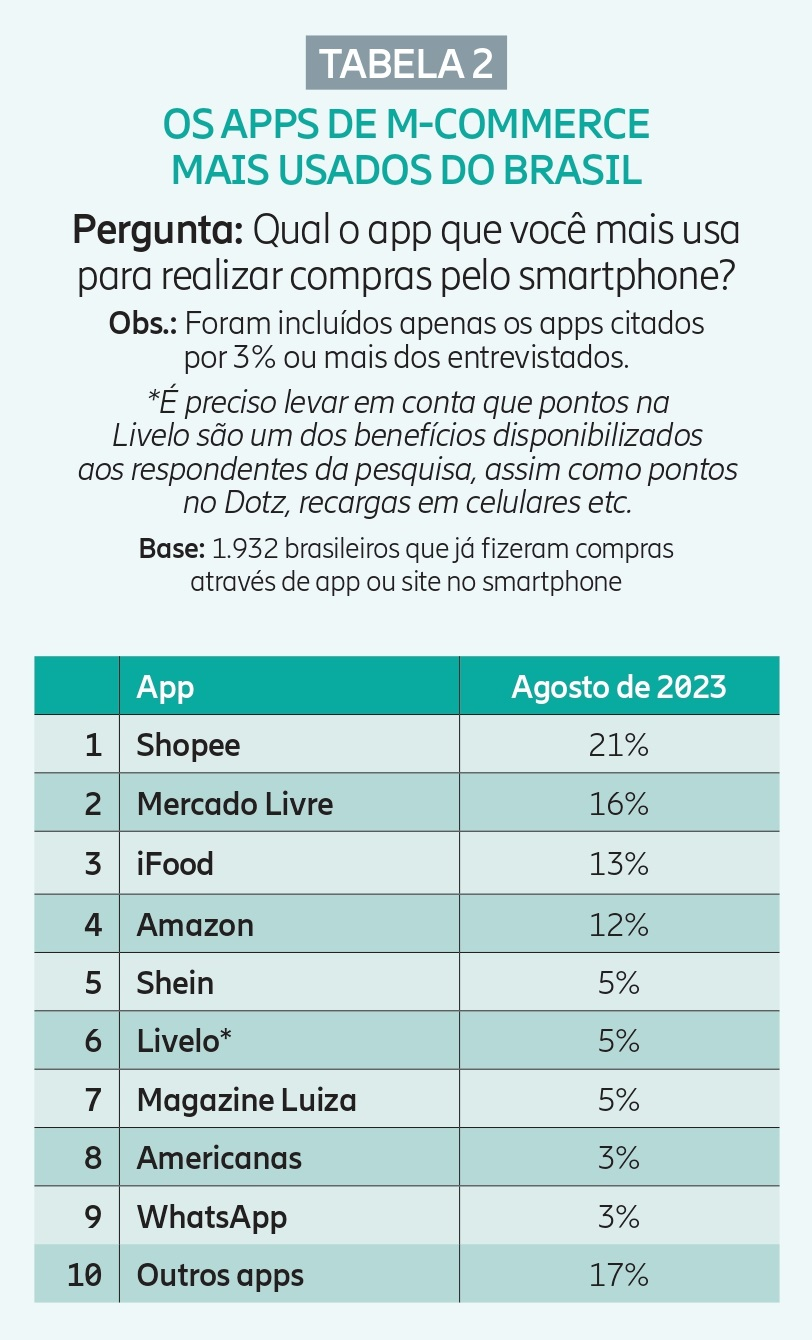
\includegraphics[keepaspectratio=true,scale=0.9]{figuras/cap05mcommerce.jpg}
    \legend{Fonte: \cite{PesquisaMCommerce}}
    \label{aplim}
\end{figure}

Após uma análise entre as duas aplicações mais utilizadas, Mercado Livre e Shopee, o foco deste estudo será explorar e aplicar boas práticas de Usabilidade no aplicativo da Shopee, orientando-se pelo viés da Experiência de Usuário. A decisão deu-se devido ao fato do Mercado Livre investir bastante em Experiência de Usuário e Usabilidade, sendo possível encontrar manuais de boas práticas em seu site institucional \cite{MercadoPagoCheck}. A própria equipe de Experiência de Usuário da empresa possui site, perfil e portfólio, que são atualizados mostrando pesquisas e melhorias feitas, com resultados apresentados centrados em métricas de Usabilidade. Por isso, a Shopee é a aplicação de Comércio Eletrônico Móvel escolhida pela autora e utilizada nesse estudo exploratório.

O comércio móvel, que consiste nas compras de produtos através de aplicativos e sites móveis, continua a crescer no Brasil. 94\% dos brasileiros com \textit{smartphone} já realizaram compras por meio de aplicativos ou sites móveis em algum momento de suas vidas, mantendo-se estável dentro da margem de erro em comparação com seis meses atrás, como mostra a Figura \ref{figura1}.

\begin{figure}[ht]
    \centering
    \caption{Frequência de Compra por Aplicativo ou Site Movel}
    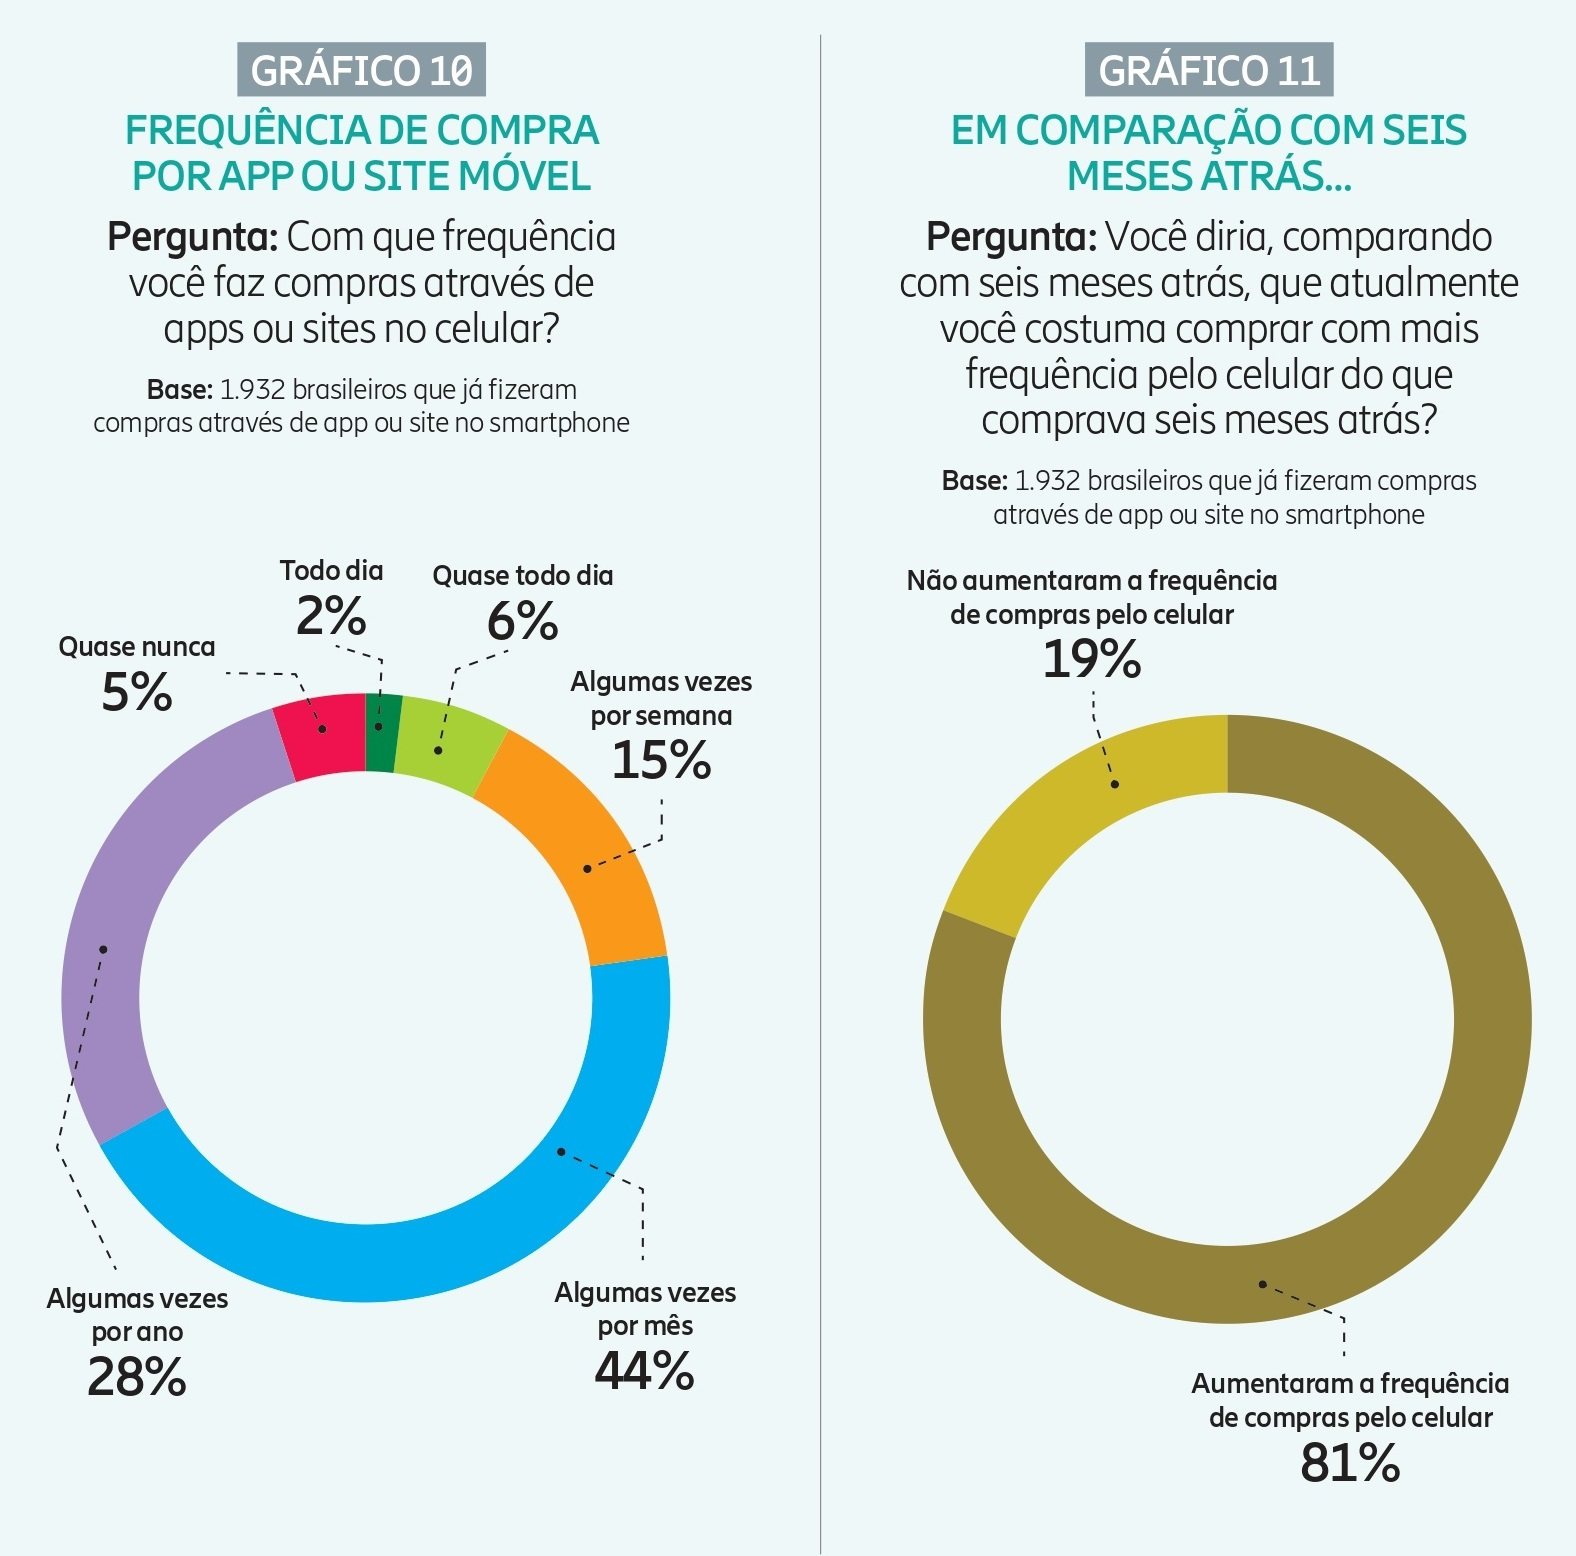
\includegraphics[keepaspectratio=true,scale=0.9]{figuras/cap05graficos1.jpg}
    \legend{Fonte: Autora}
    \label{figura1}
\end{figure}

Considerando que a aplicação já existe e está em uso há bastante tempo, para a implementação das melhorias de Usabilidade orientadas à Experiência de Usuário, foram consideradas as Heurísticas de Nielsen, assim como guias mencionados ao longo deste trabalho, como os próprios princípios heurísticos para interfaces móveis. Ambos, heurísticas de Nielsen e princípios heurísticos para interfaces móveis, foram apresentados no \hyperref[chap:ReferencialTeorico]{Capítulo 2 - Referencial Teórico}, seções \ref{HeuristicasNielsen} e \ref{HeuristicasMoveis}. Para a primeira parte do trabalho, através de pesquisas e questionários, tem sido realizada, já com resultados sendo apresentados nessa monografia, uma análise geral da aplicação Shopee. A intenção principal é procurar apontar as principais dificuldades encontradas pelos usuários, em alguns fluxos de tela. Já na segunda parte deste estudo, será feito um acompanhamento mais detalhado com testes de usabilidade e protótipos de alta fidelidade, aplicando melhorias diretas na interface da aplicação.

A fim de conhecer a aplicação escolhida, e já conferir uma visão mais concreta sobre o andamento desse estudo, foi realizada uma prova de conceito, desde essa primeira etapa do trabalho.

\section{Prova de Conceito}
    \label{ProvaConceito}

Para este TCC, a Prova de Conceito assume um papel relevante ao testar as hipóteses formuladas sobre as melhorias propostas na Experiência do Usuário. Essas melhorias podem abranger aspectos como usabilidade, acessibilidade, desempenho e outros elementos que afetam a percepção e a satisfação do usuário ao interagir com um sistema, produto ou serviço.

Segundo a Revista da Faculdade de Direito de Campo (2004), uma prova de conceito consiste em um modelo de cunho prático, que procura provar um conceito teórico, advindo da literatura especializada, apresentando insumos mais concretos. Por vezes, é incompleta ou sucinta. Durante a execução da Prova de Conceito, é essencial manter um registro detalhado das observações, \textit{feedbacks} e resultados obtidos. Isso permite uma análise criteriosa dos dados coletados para determinar se as melhorias propostas alcançaram os objetivos estabelecidos. Além disso, a Prova de Conceito oferece \textit{insights} valiosos que podem orientar ajustes finais e refinamentos antes da implementação completa das melhorias \cite{ProvaConceito}.

No caso do presente trabalho, a prova de conceito foi realizada com base na aplicação Shopee, consistindo em levantar insumos que comprovem a popularidade da mesma, além de maior conhecimento sobre a versão mais atualizada dessa aplicação e possibilidades de melhorias.

\section{Shopee}
    \label{Shopee}
    
A Shopee é uma plataforma de comércio eletrônico fundada em 2015 em Singapura e pertencente ao Grupo \textit{Sea Limited}. Opera como um \textit{marketplace}, conectando vendedores e compradores em uma ampla variedade de categorias de produtos, incluindo eletrônicos, moda, beleza, casa e decoração, entre outros. A plataforma oferece uma experiência de compra conveniente, com recursos como frete grátis, promoções e descontos, além de opções de pagamento seguras e diversas. A Shopee também promove ativamente o envolvimento dos usuários por meio de recursos de gamificação, como jogos e competições, para melhorar a experiência do usuário e promover a fidelidade à marca.

Como mencionado anteriormente, a plataforma possui uma ampla variedade de produtos à venda, o que torna o público-alvo bastante diverso, pois atualmente grande parte da população possui acesso à internet. A seguir, são apresentadas algumas particularidades da versão atual dessa aplicação.

\subsection{Versão Atual da Aplicação}

Segundo levantamentos realizados pela autora do presente trabalho, a aplicação Shopee possui falhas em seus fluxos, considerando a Usabilidade, que podem ser percebidas pelos seus usuários, quando interagem com essa plataforma de Comércio Eletrônico Móvel. O intuito é ilustrar sobre essas falhas, até mesmo em fluxos considerados simples, e que são identificadas pelos usuários enquanto navegam pela aplicação Shopee. Tais falhas foram identificadas e selecionadas usando como base os comentários avaliativos da aplicação Shopee, como exemplificado na Figura \ref{s0}. Além de apresentar pontos de melhoria para cada situação, como alguns dos insumos de relevância deste trabalho são os protótipos de alta fidelidade aplicando boas práticas na interface da aplicação Shopee, as melhorias são apresentadas de forma mais teórica do que prática. A ideia é conferir, nesse primeiro momento, apenas evidências sobre a ocorrência de erros na aplicação, para assim aplicar melhorias em uma segunda etapa do estudo.

\begin{figure}[ht]
    \centering
    \caption{Opinião do Público sobre a Shopee via PlayStore}
    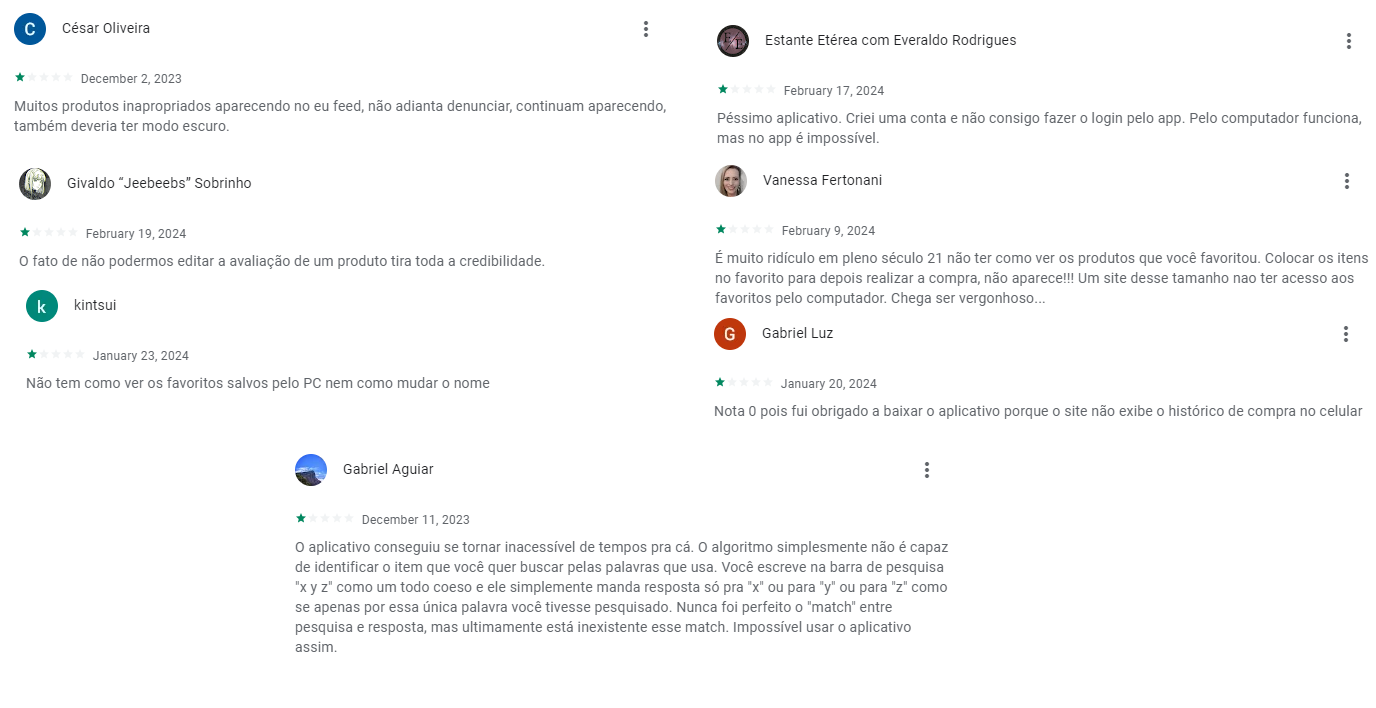
\includegraphics[keepaspectratio=true,scale=0.3]{figuras/cap05shopee.PNG}
    \legend{Fonte: Autora}
    \label{s0}
\end{figure}

Na Figura \ref{s1}, é possível perceber como a visualização do rastreamento de um produto já incorre em não atendimento da primeira Heurística estabelecida por Nielsen. Não existe visibilidade do status ou um \textit{feedback} imediato do andamento. Sendo assim, o usuário acaba sempre precisando percorrer muitos passos para ter acesso à informação. Adicionalmente, cabe ressaltar que a forma de exposição não é dinâmica, nem mesmo atrativa ao usuário.

\begin{figure}[ht]
    \centering
    \caption{Rastreamento do Produto pela Shopee}
    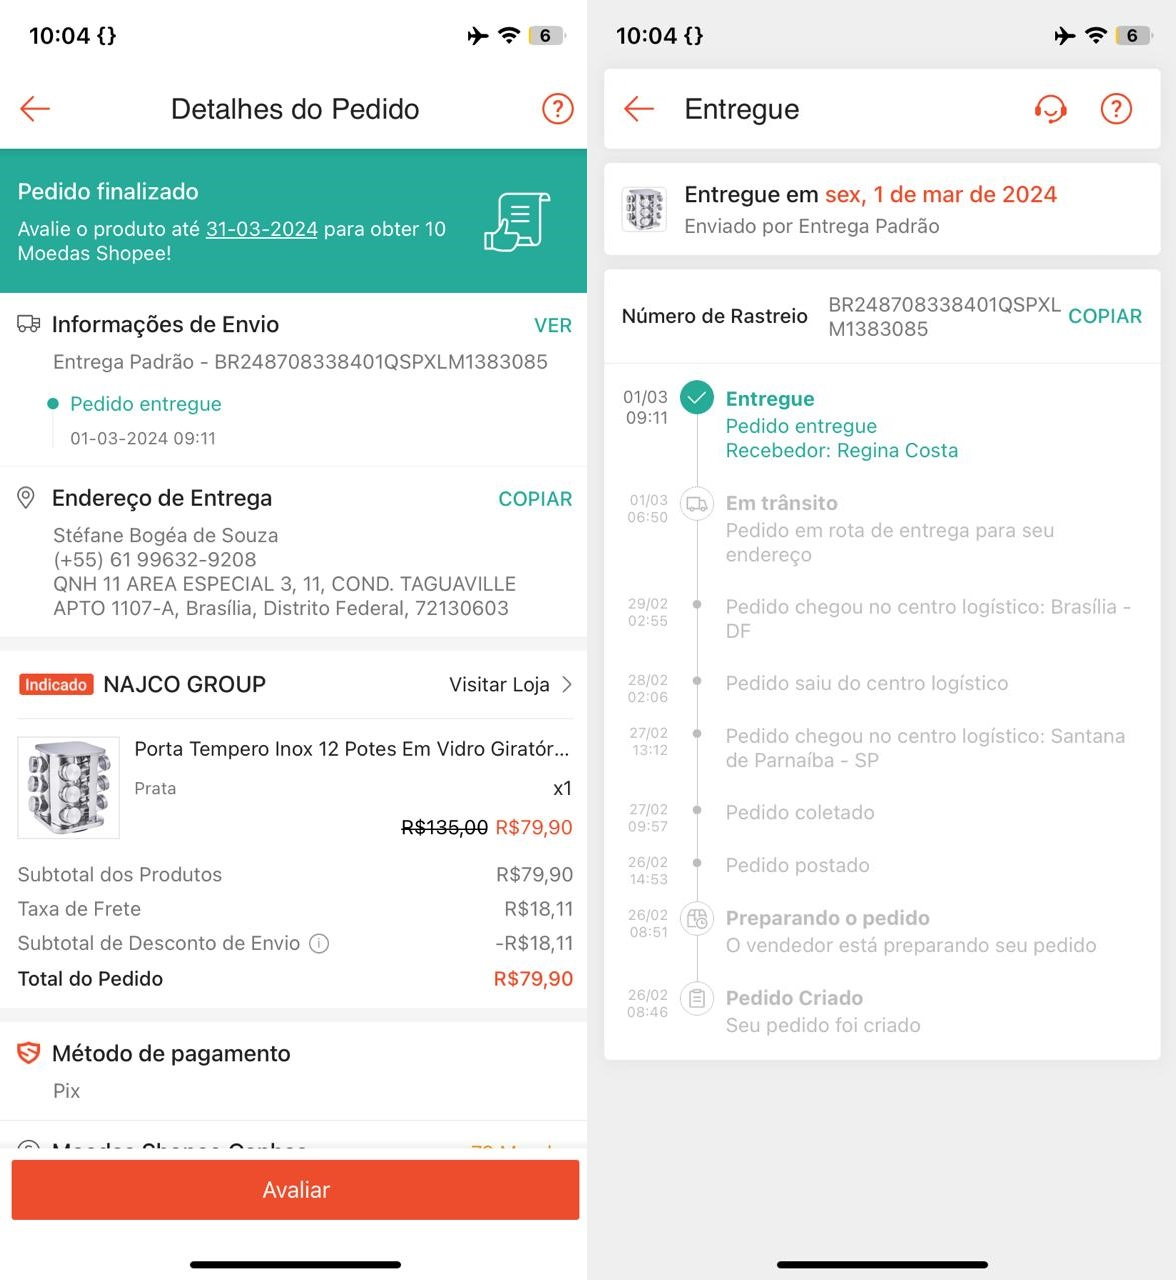
\includegraphics[keepaspectratio=true,scale=0.3]{figuras/shopeeRas.jpg}
    \legend{Fonte: Autora}
    \label{s1}
\end{figure}

Na Figura \ref{s2}, é mostrado o fluxo de devolução de um produto, no qual foi solicitado o reembolso e disponibilizadas as instruções de como devolver o produto. Existem aspectos bons, como a barra de progresso na parte superior, indicando ao usuário como está o andamento do processo. Entretanto, a informação é colocada ao usuário como um longo texto, sem elementos visuais que facilitem o entendimento. Uma sugestão de melhoria pode ser encontrada na Figura \ref{melhoria}, onde consta uma tela bem mais simples e agradável aos olhos dos usuários.

\begin{figure}[ht]
    \centering
    \caption{Processo de Devolução pela Shopee}
    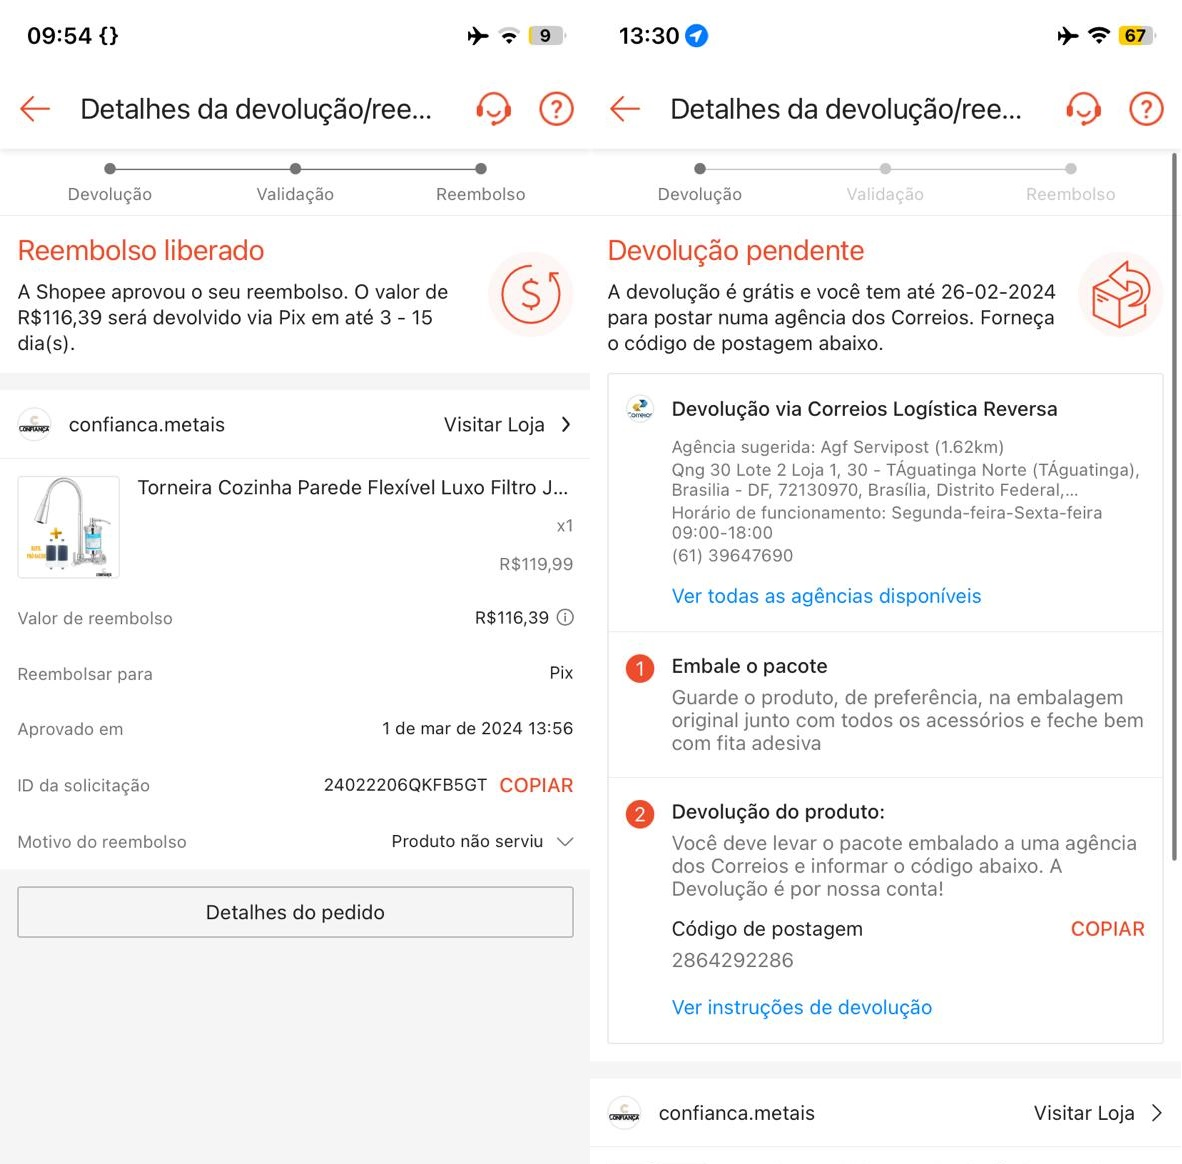
\includegraphics[keepaspectratio=true,scale=0.3]{figuras/shopee2.jpg}
    \legend{Fonte: Autora}
    \label{s2}
\end{figure}

\begin{figure}[ht]
    \centering
    \caption{Sugestão de Melhoria para Interface de Devolução}
    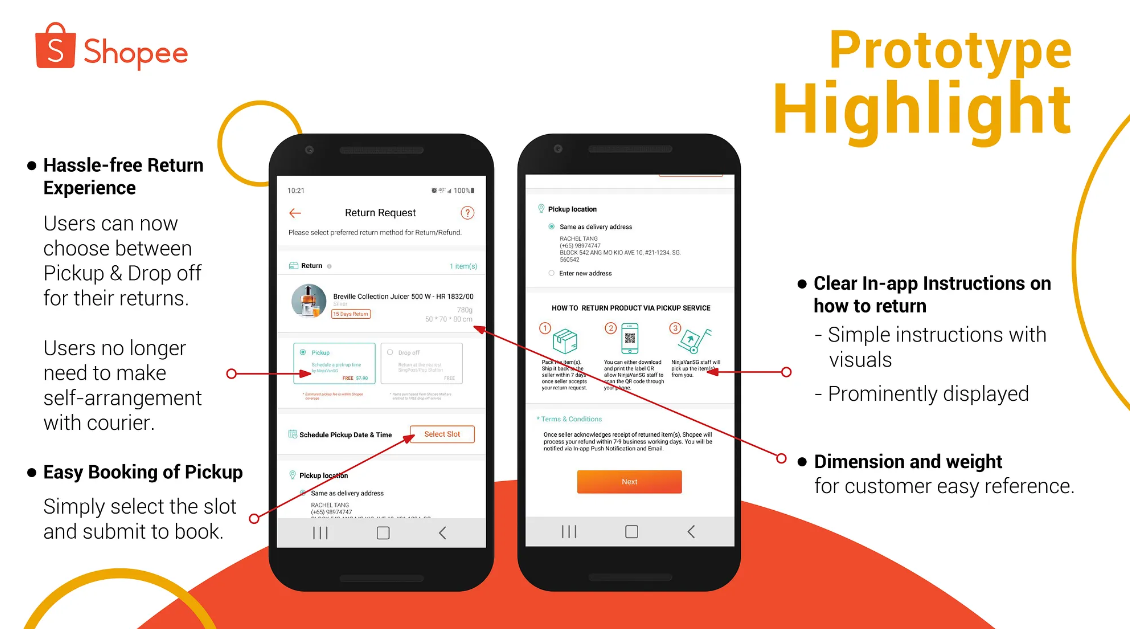
\includegraphics[keepaspectratio=true,scale=0.3]{figuras/melhoria.PNG}
    \legend{Fonte: Lim Evelyn. Disponível em: <https://lbh-evelyn.medium.com/shopee-app-ux-case-study-6938d323d5df>}
    \label{melhoria}
\end{figure}

Na Figura \ref{s3}, o perfil da loja Cacau Show pode ser visualizado. Contudo, informações importantes, como avaliações da loja, taxa de resposta, tempo de servio na plataforma, entre outros, só são disponibilizadas ao clicar em outra tela. Segundo a pesquisa \citeonline{PesquisaMCommerce}, um dos fatores mais importantes para o usuário no momento de escolher seu produto ou pesquisar uma nova loja é justamente informações que transmitam confiabilidade na loja. Assim, a taxa de desistência de compra pode tender ao aumento pelo simples fato de não terem sido expostas ao cliente informações essenciais do negócio.

\begin{figure}[ht]
    \centering
    \caption{Perfil da Loja Cacau Show na Shopee}
    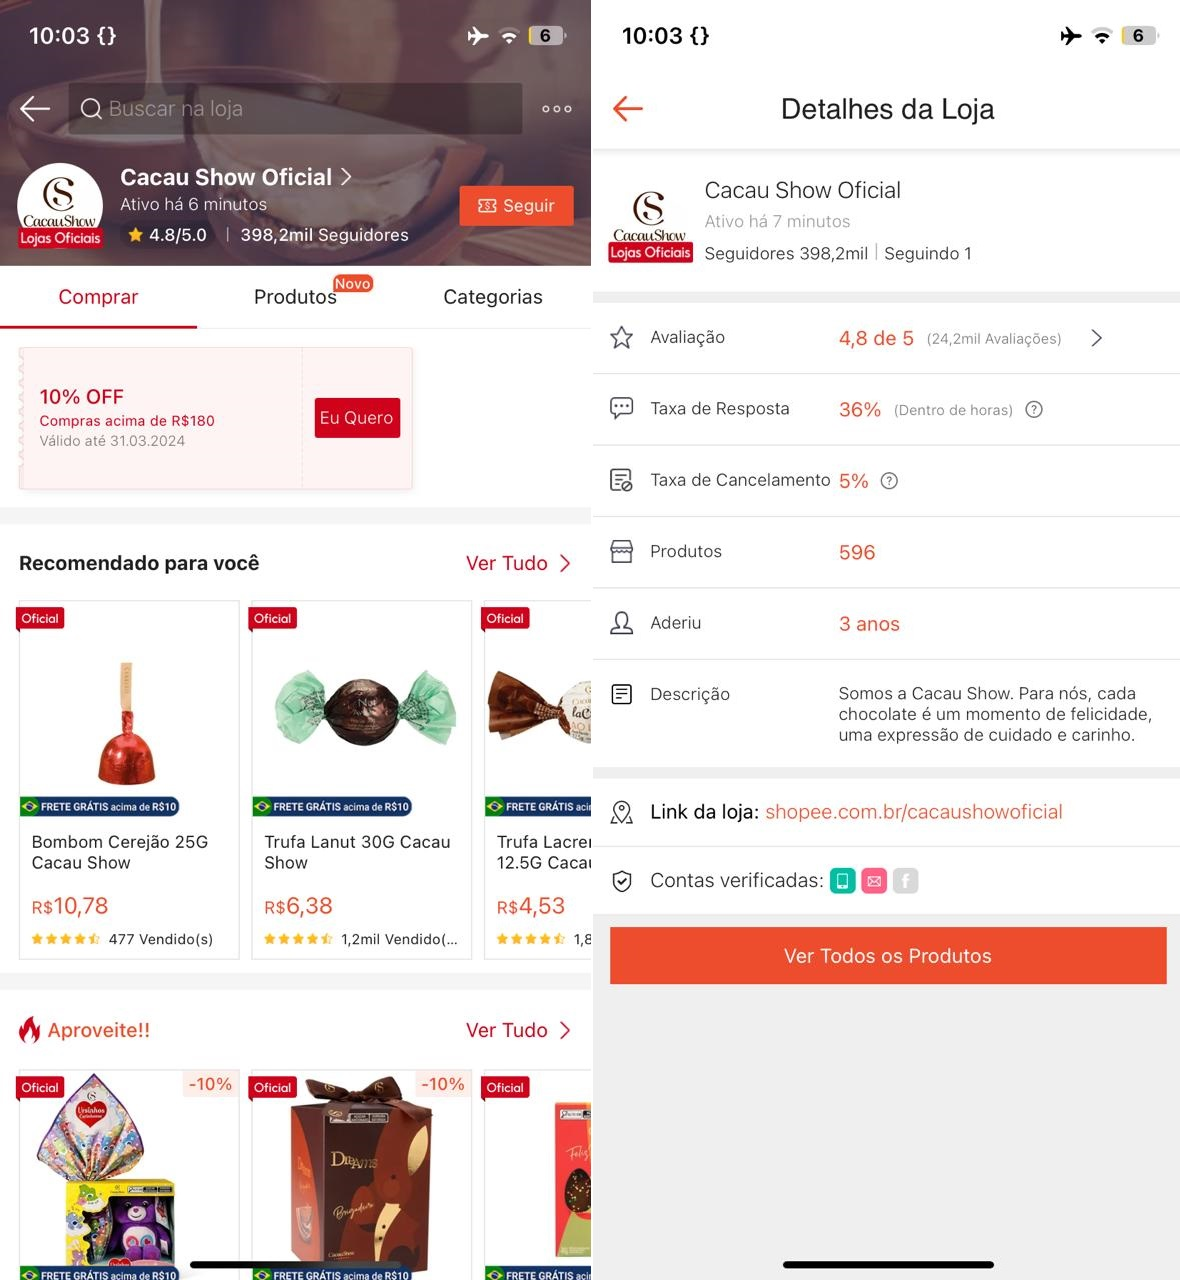
\includegraphics[keepaspectratio=true,scale=0.3]{figuras/shopee3.jpg}
    \legend{Fonte: Autora}
    \label{s3}
\end{figure}

Na Figura \ref{s4}, é ilustrado o fluxo de compra, com notificações e avaliações do usuário. É possível analisar que a interface do aplicativo é sempre repleta de informações, confusa, deixando o usuário cansado apenas de olhar, sem saber exatamente focar ou considerar prioritário. Na interface de notificações, por exemplo, seria muito interessante tirar a pré-visualização das mensagens, deixando apenas o ícone de mensagem não lida. Isso permitiria uma interface mais agradável ao usuário, além de visualmente limpa. Como \citeonline{HeuristicasResumo} cita em um estudo voltando às Heuristicas de Nielsen para interfaces móveis. Nesse contexto, a Limitação de Informação e Estética do \textit{Design} são importantes, precisando ter cuidado com a tipografia, bem como com o excesso de informações, dentre outros aspectos. O mesmo pode ser aplicado para interface do Carrinho, na qual os produtos são colocados em forma de lista, sem elemento visual algum, para que o usuário possa perceber que está comprando itens de lojas diferentes.

\begin{figure}[ht]
    \centering
    \caption{Fluxo de Compra, Notificação e Avaliação de Compra na Shopee}
    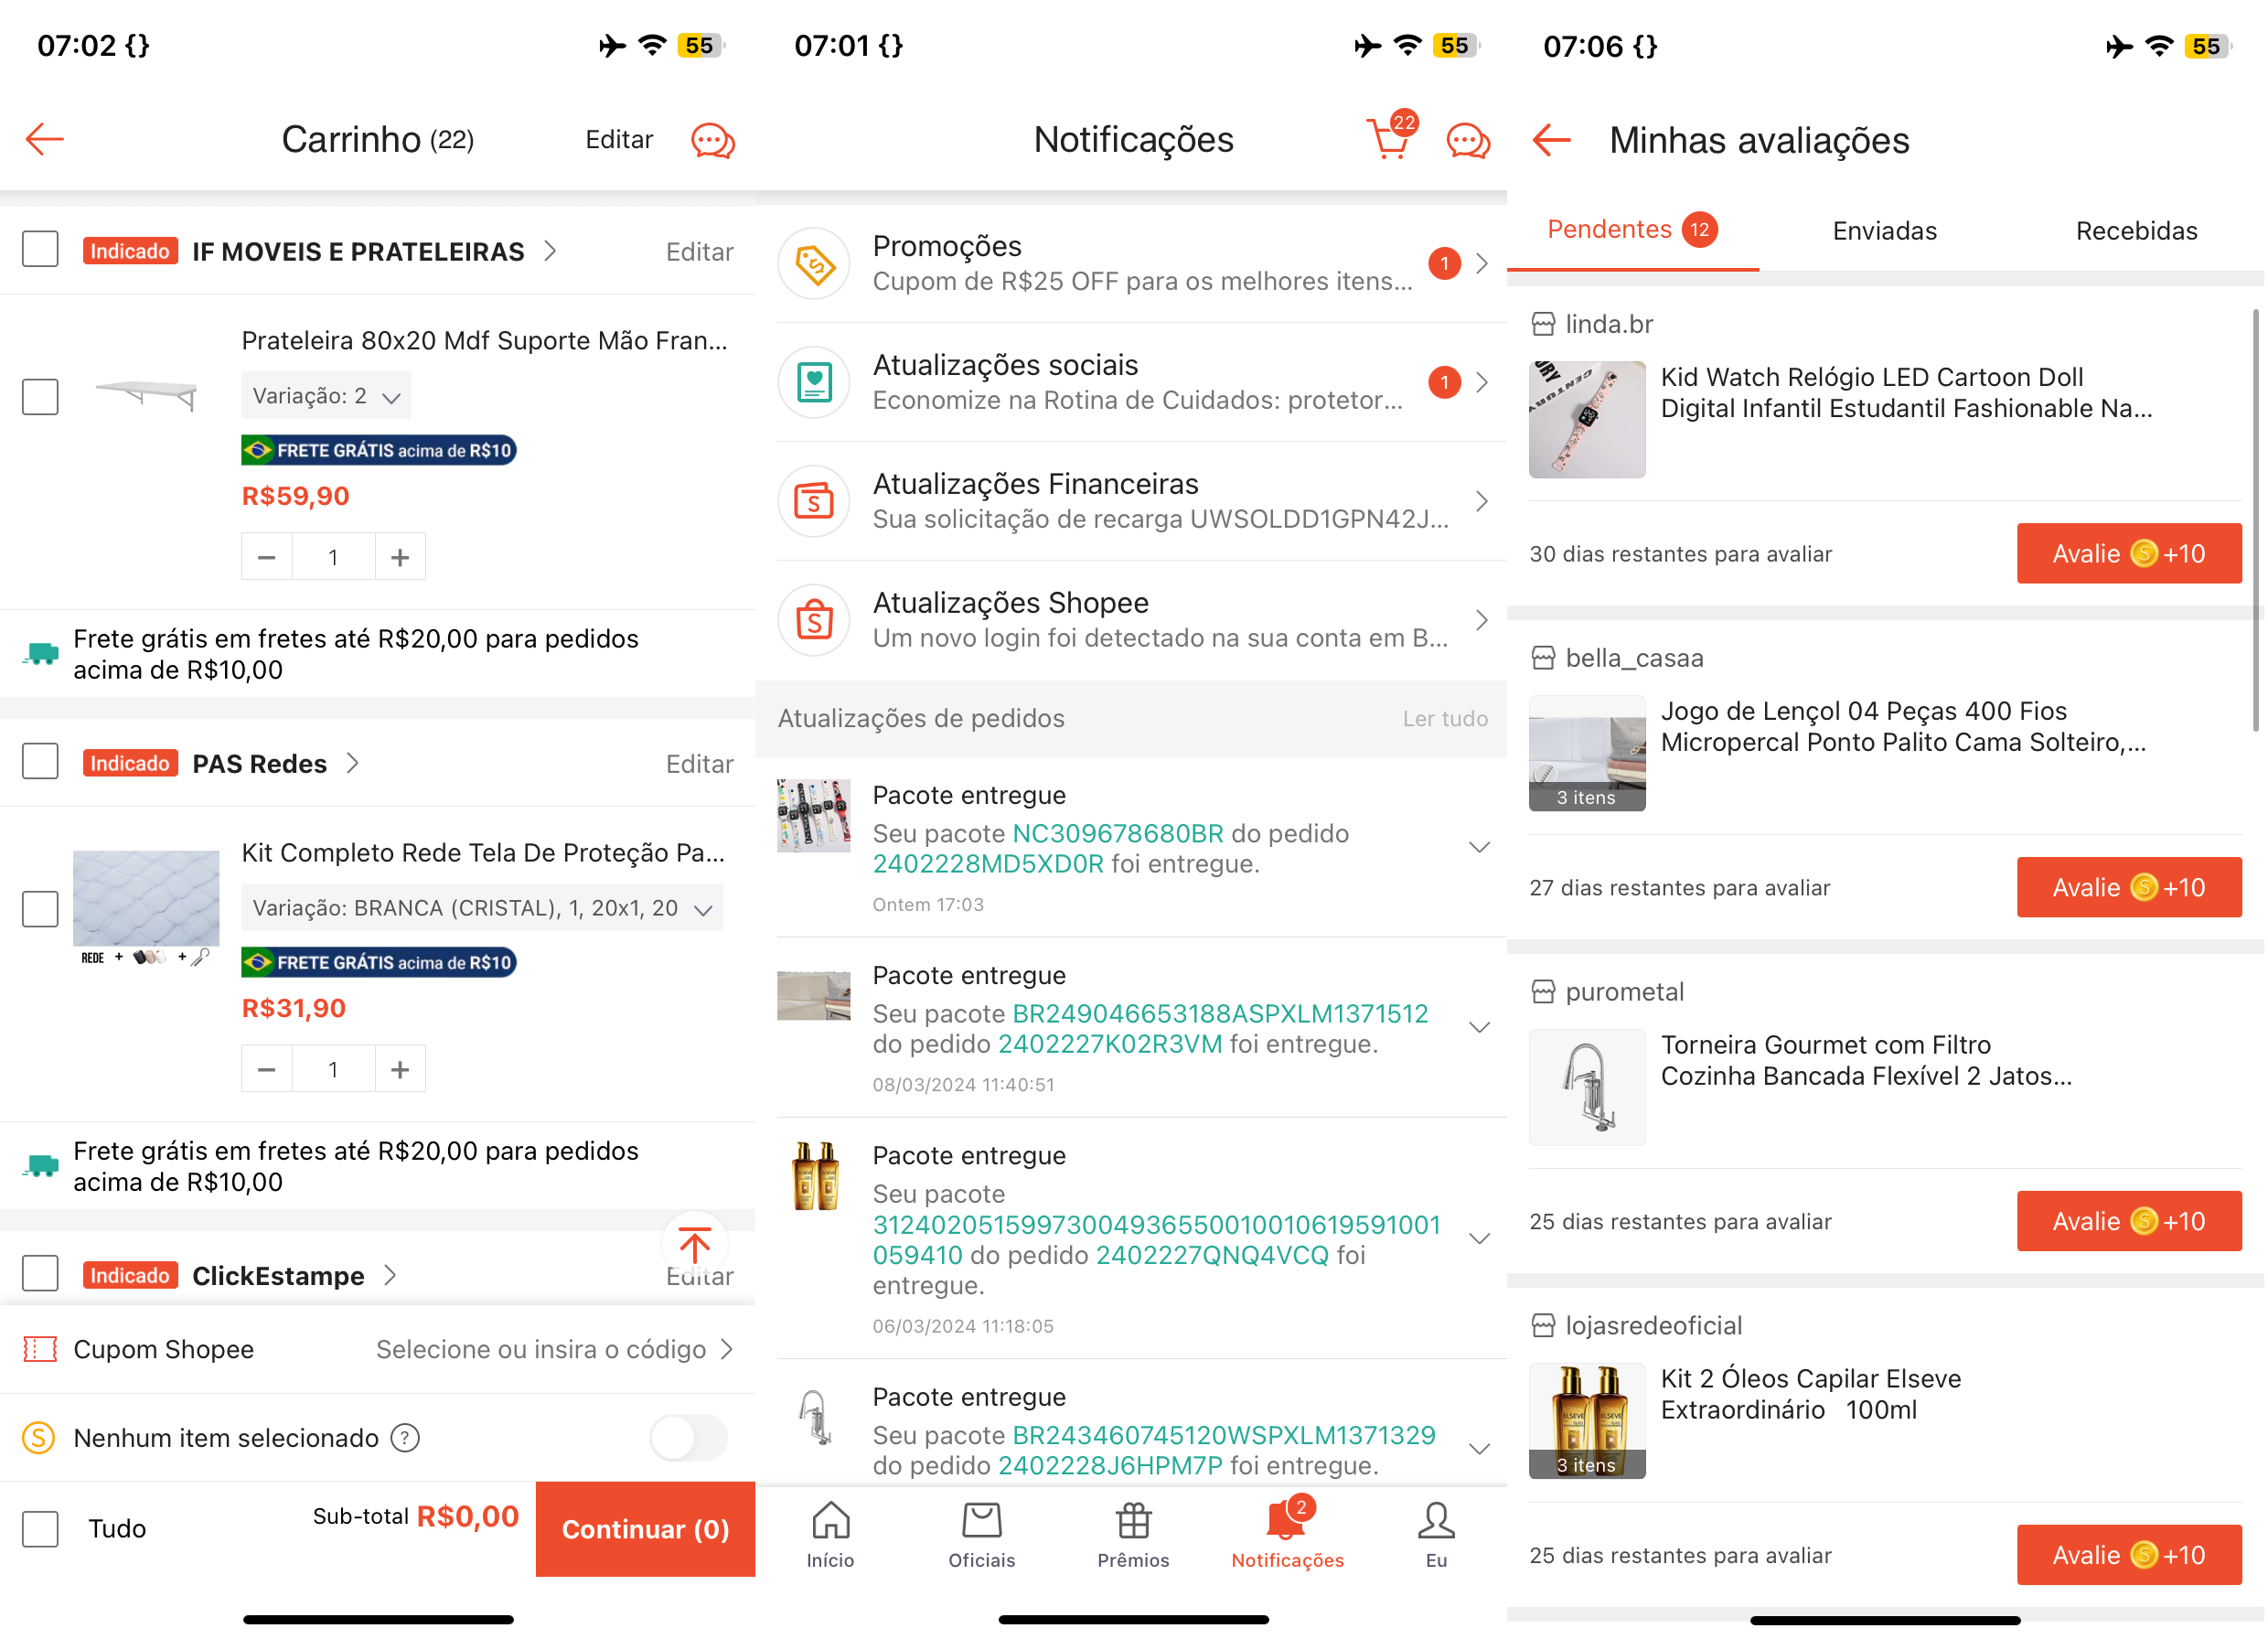
\includegraphics[keepaspectratio=true,scale=0.2]{figuras/shopee4.PNG}
    \legend{Fonte: Autora}
    \label{s4}
\end{figure}

Na Figura \ref{s5}, tem-se o excesso de informações na tela principal, e uma busca mal sucedida no aplicativo apesar de palavras-chave corretas. Novamente, a aplicação falha em entregar ao usuário um ambiente não necessariamente minimalista, ou seja, visualmente organizado e sem repetições desnecessárias. Por exemplo, na tela inicial, tem-se a barra de pesquisa com nome de produtos sugeridos, sendo que esse mesmo produto já está exposto no \textit{banner} "Melhores Preços da Semana", que também falha em não apresentar mais opções ao usuário limitando-se à apenas três seleções de produtos sem classificação por categoria.

Na Figura \ref{s5}, os botões, apresentados logo abaixo do \textit{frame} de topo da interface, são redundantes. Funcionalidades, como "Moedas e Prêmios", "Cupons", "\textit{ShopeePay}", poderiam ser agrupadas. Essas funcionalidades estão relacionadas à parte financeira, no contexto da aplicação. O ícone de "Lojas Oficiais" e "Prêmios" aparece duas vezes na mesma tela, uma entre as opções logo na entrada e novamente na barra inferior da aplicação, causando confusão e complexidade visual ao usuário. Como o ícone de "Moedas", ocorre da mesma forma. Entretanto, com a diferença que esse aparece pela segunda vez como uma mensagem flutuante, perto do menu inferior.

A seção "Ofertas Relâmpago" não oferece qualquer informação sobre qualquer produto. A proposta, como o nome estabelece, entende-se ser algo rápido e passageiro, incentivando o usuário à compra. Contudo, não existem informações sobre o produto, tais como nome, categoria e versão. Assim, força o usuário a clicar no produto para verificar mesmo que não seja o que procura, causando frustração.

Por fim, a ferramenta de busca exibe informações contrárias às que o usuário procura, orientando-se por uma seleção de palavras por palavra, e não considerando o termo desejado na busca como fazendo parte de uma composição de palavras. Quando realizada a busca, novamente mais frustração para o usuário que, além de não encontrar o que deseja nos primeiros resultados, precisa deslizar a tela, encontrando ainda opções de filtro confusas.

\begin{figure}[ht]
    \centering
    \caption{Página Principal do aplicativo da Shopee}
    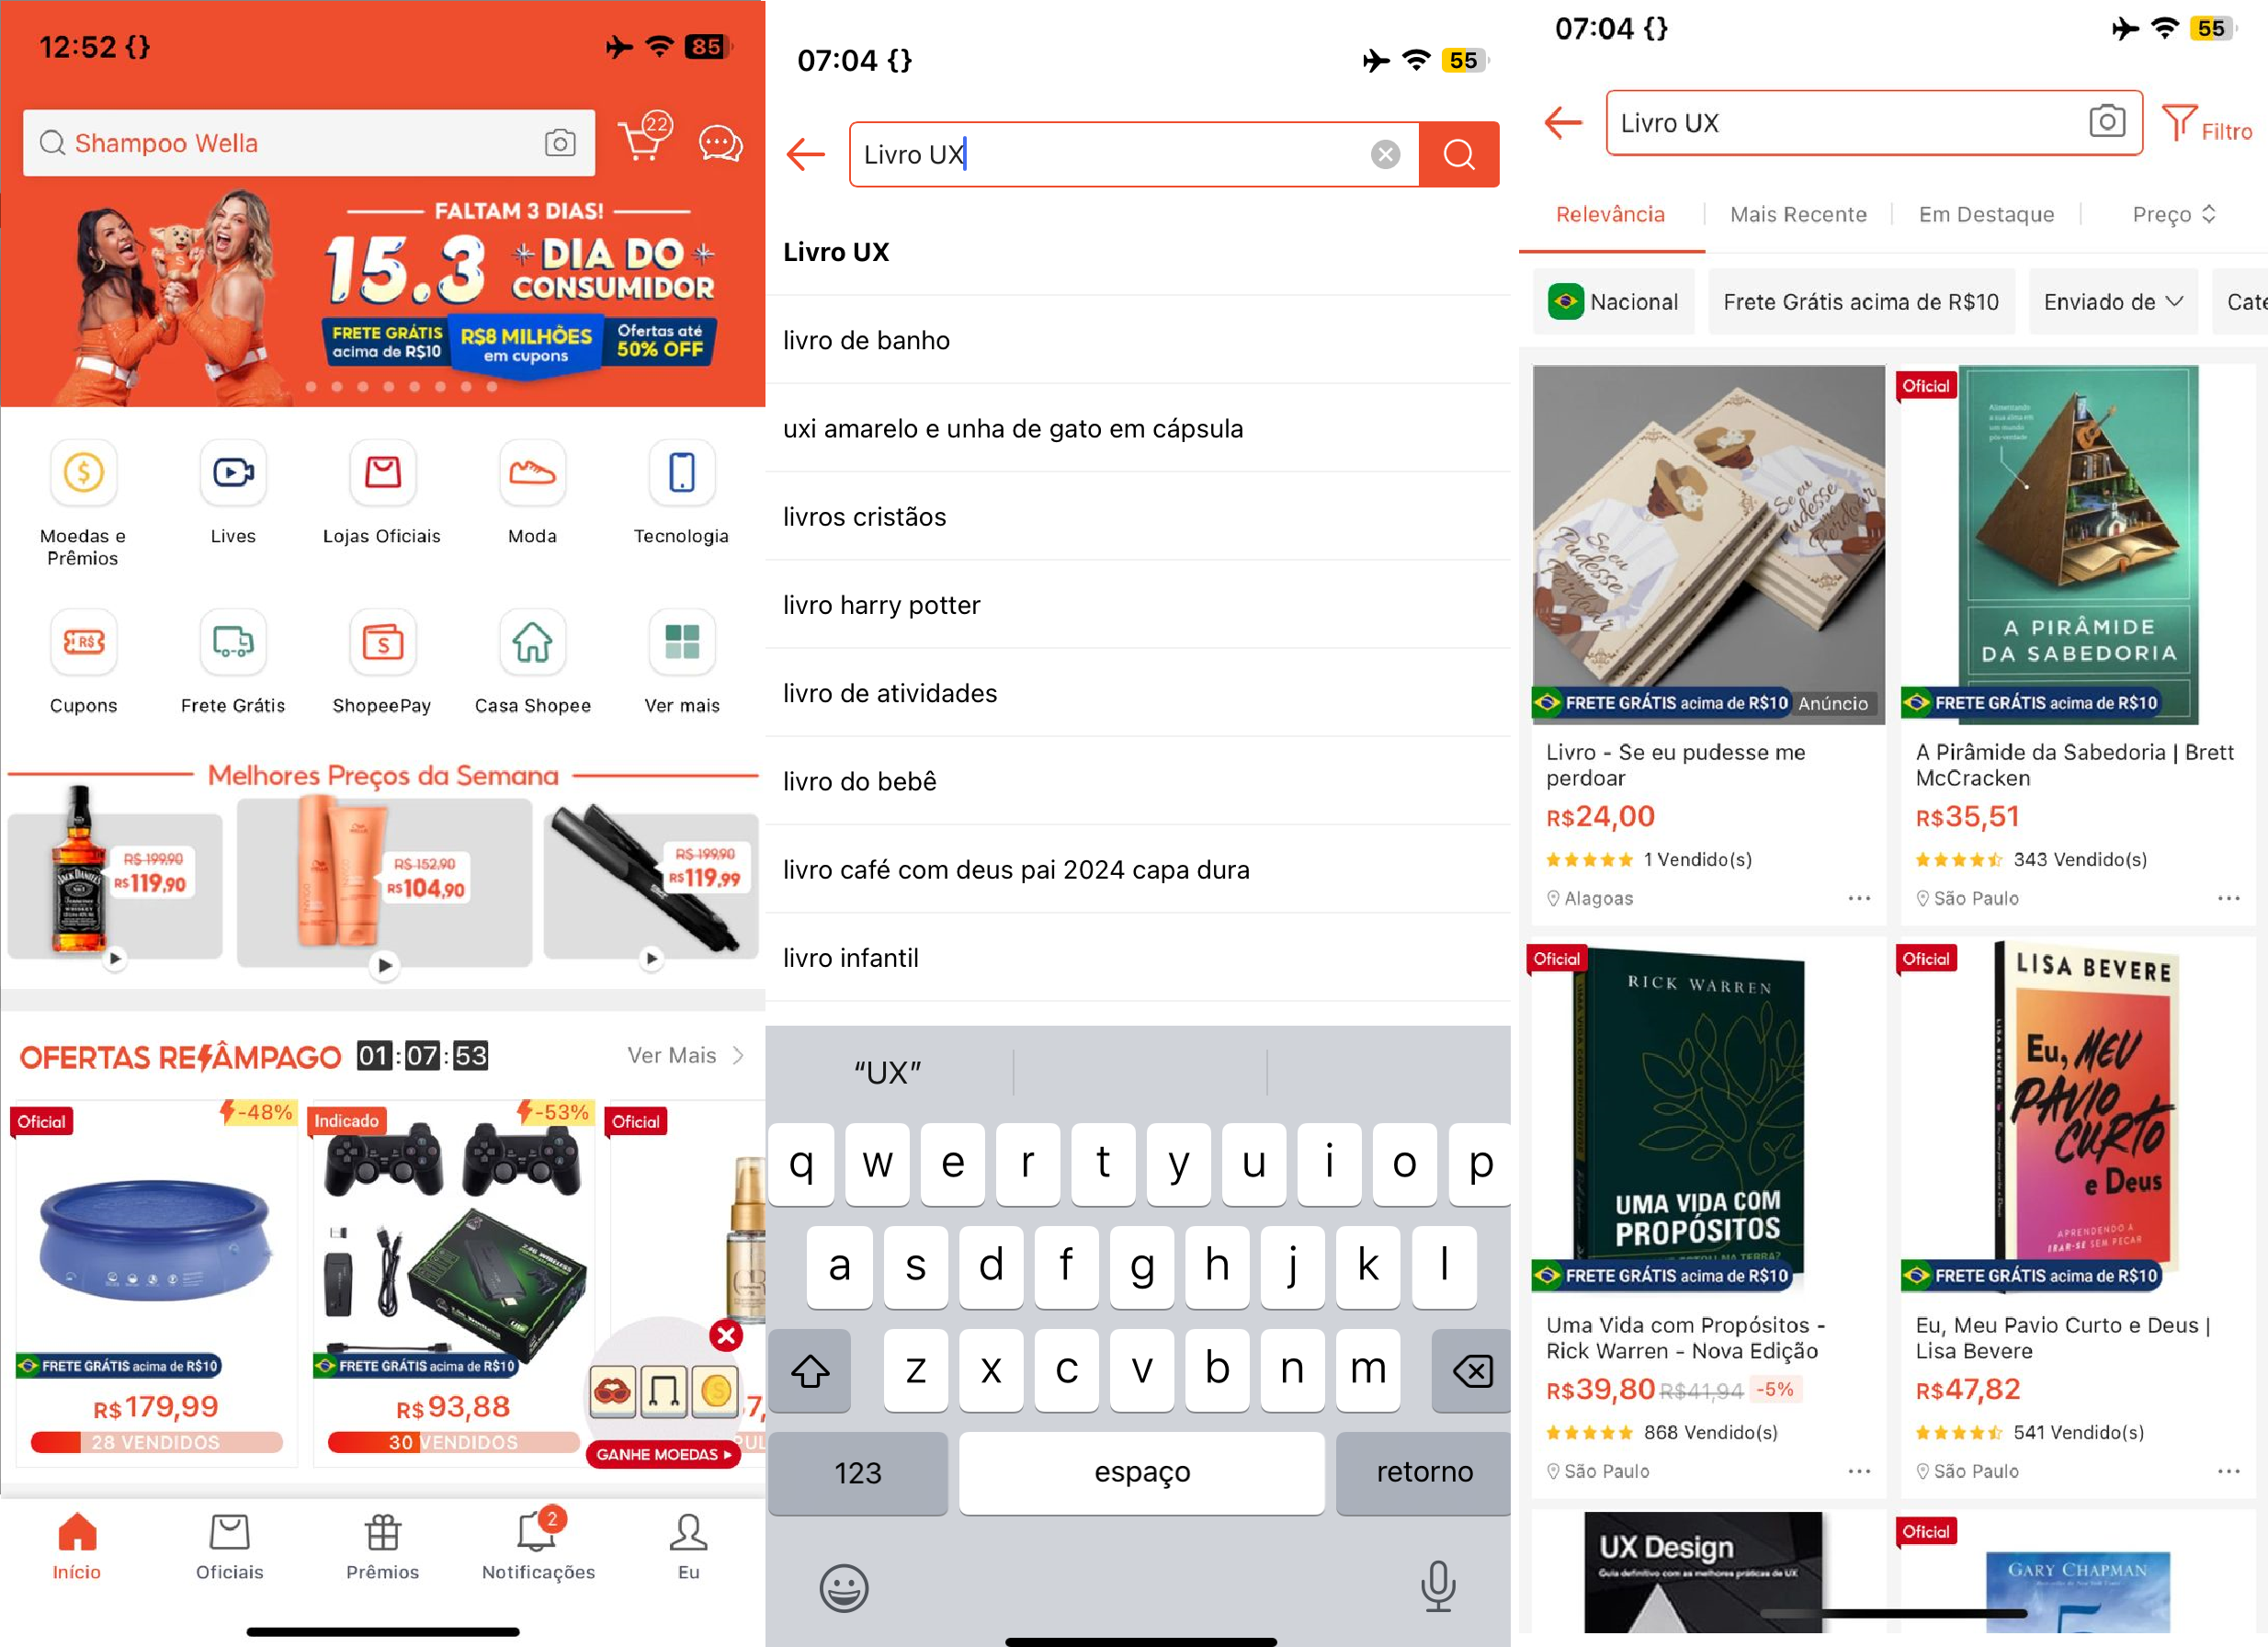
\includegraphics[keepaspectratio=true,scale=0.2]{figuras/shopee1.PNG}
    \legend{Fonte: Autora}
    \label{s5}
\end{figure}

\subsection{Análise do Questionário Aplicado}
    \label{AnaliseAttrakDiffR}

Para iniciar as análises das principais aplicações de Comércio Eletrônico Móvel, foi aplicado um questionário baseado nas métricas de análise do \textit{AttrakDiff-R}. Como o objetivo deste primeiro contato com os usuários pretendia ser mais amplo, nenhuma funcionalidade foi avaliada de forma isolada. O questionário tinha como objetivo alinhar seus resultados com as pesquisas feitas por \citeonline{PesquisaMCommerce} e \citeonline{ConversionDocs}, como também entender seu público geral, para assim definir possíveis Personas para um Teste de Usabilidade com foco mais específico. Adicionalmente, foi possível questionar o usuário sobre alguma funcionalidade que o mesmo teria dificuldade e/ou sentiu que necessitava de uma melhoria, baseado na aplicação mais utilizada por esse usuário.

Diante disso, foi possível analisar através de 55 participantes do questionário que o público de interesse para o domínio desse trabalho é composto quase na mesma proporção por homens e mulheres, tendo mulheres como maior participação. Em questão de idade, destaca-se um público majoritariamente entre pessoas de 20 a 50 anos. A aplicação mais utilizada entre os participantes foi a Shopee com 54,4\%, como mostra a Figura \ref{ShopeeGrafico}, tendo sua maior reclamação conferida às funcionalidades "Buscar Produtos" e "Descrever Produtos" como mostra a Figura \ref{FuncionalidadeShopee}.

\begin{figure}[ht]
    \centering
    \caption{Comércio Eletrônico Mais Utilizado com base no questionário}
    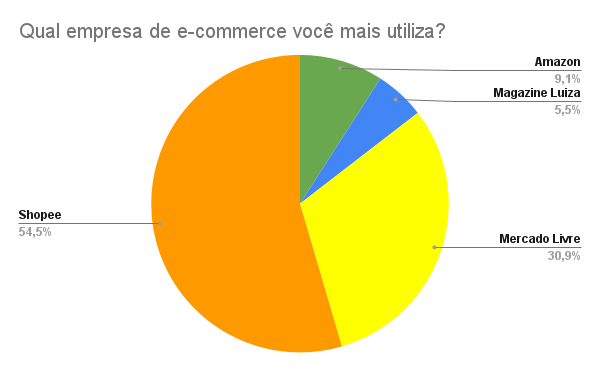
\includegraphics[keepaspectratio=true,scale=0.5]{figuras/empresa.png}
    \legend{Fonte: Autora}
    \label{ShopeeGrafico}
\end{figure}

\begin{figure}[ht]
    \centering
    \caption{Funcionalidades da Shopee que necessitam de melhoria na visão do usuário}
    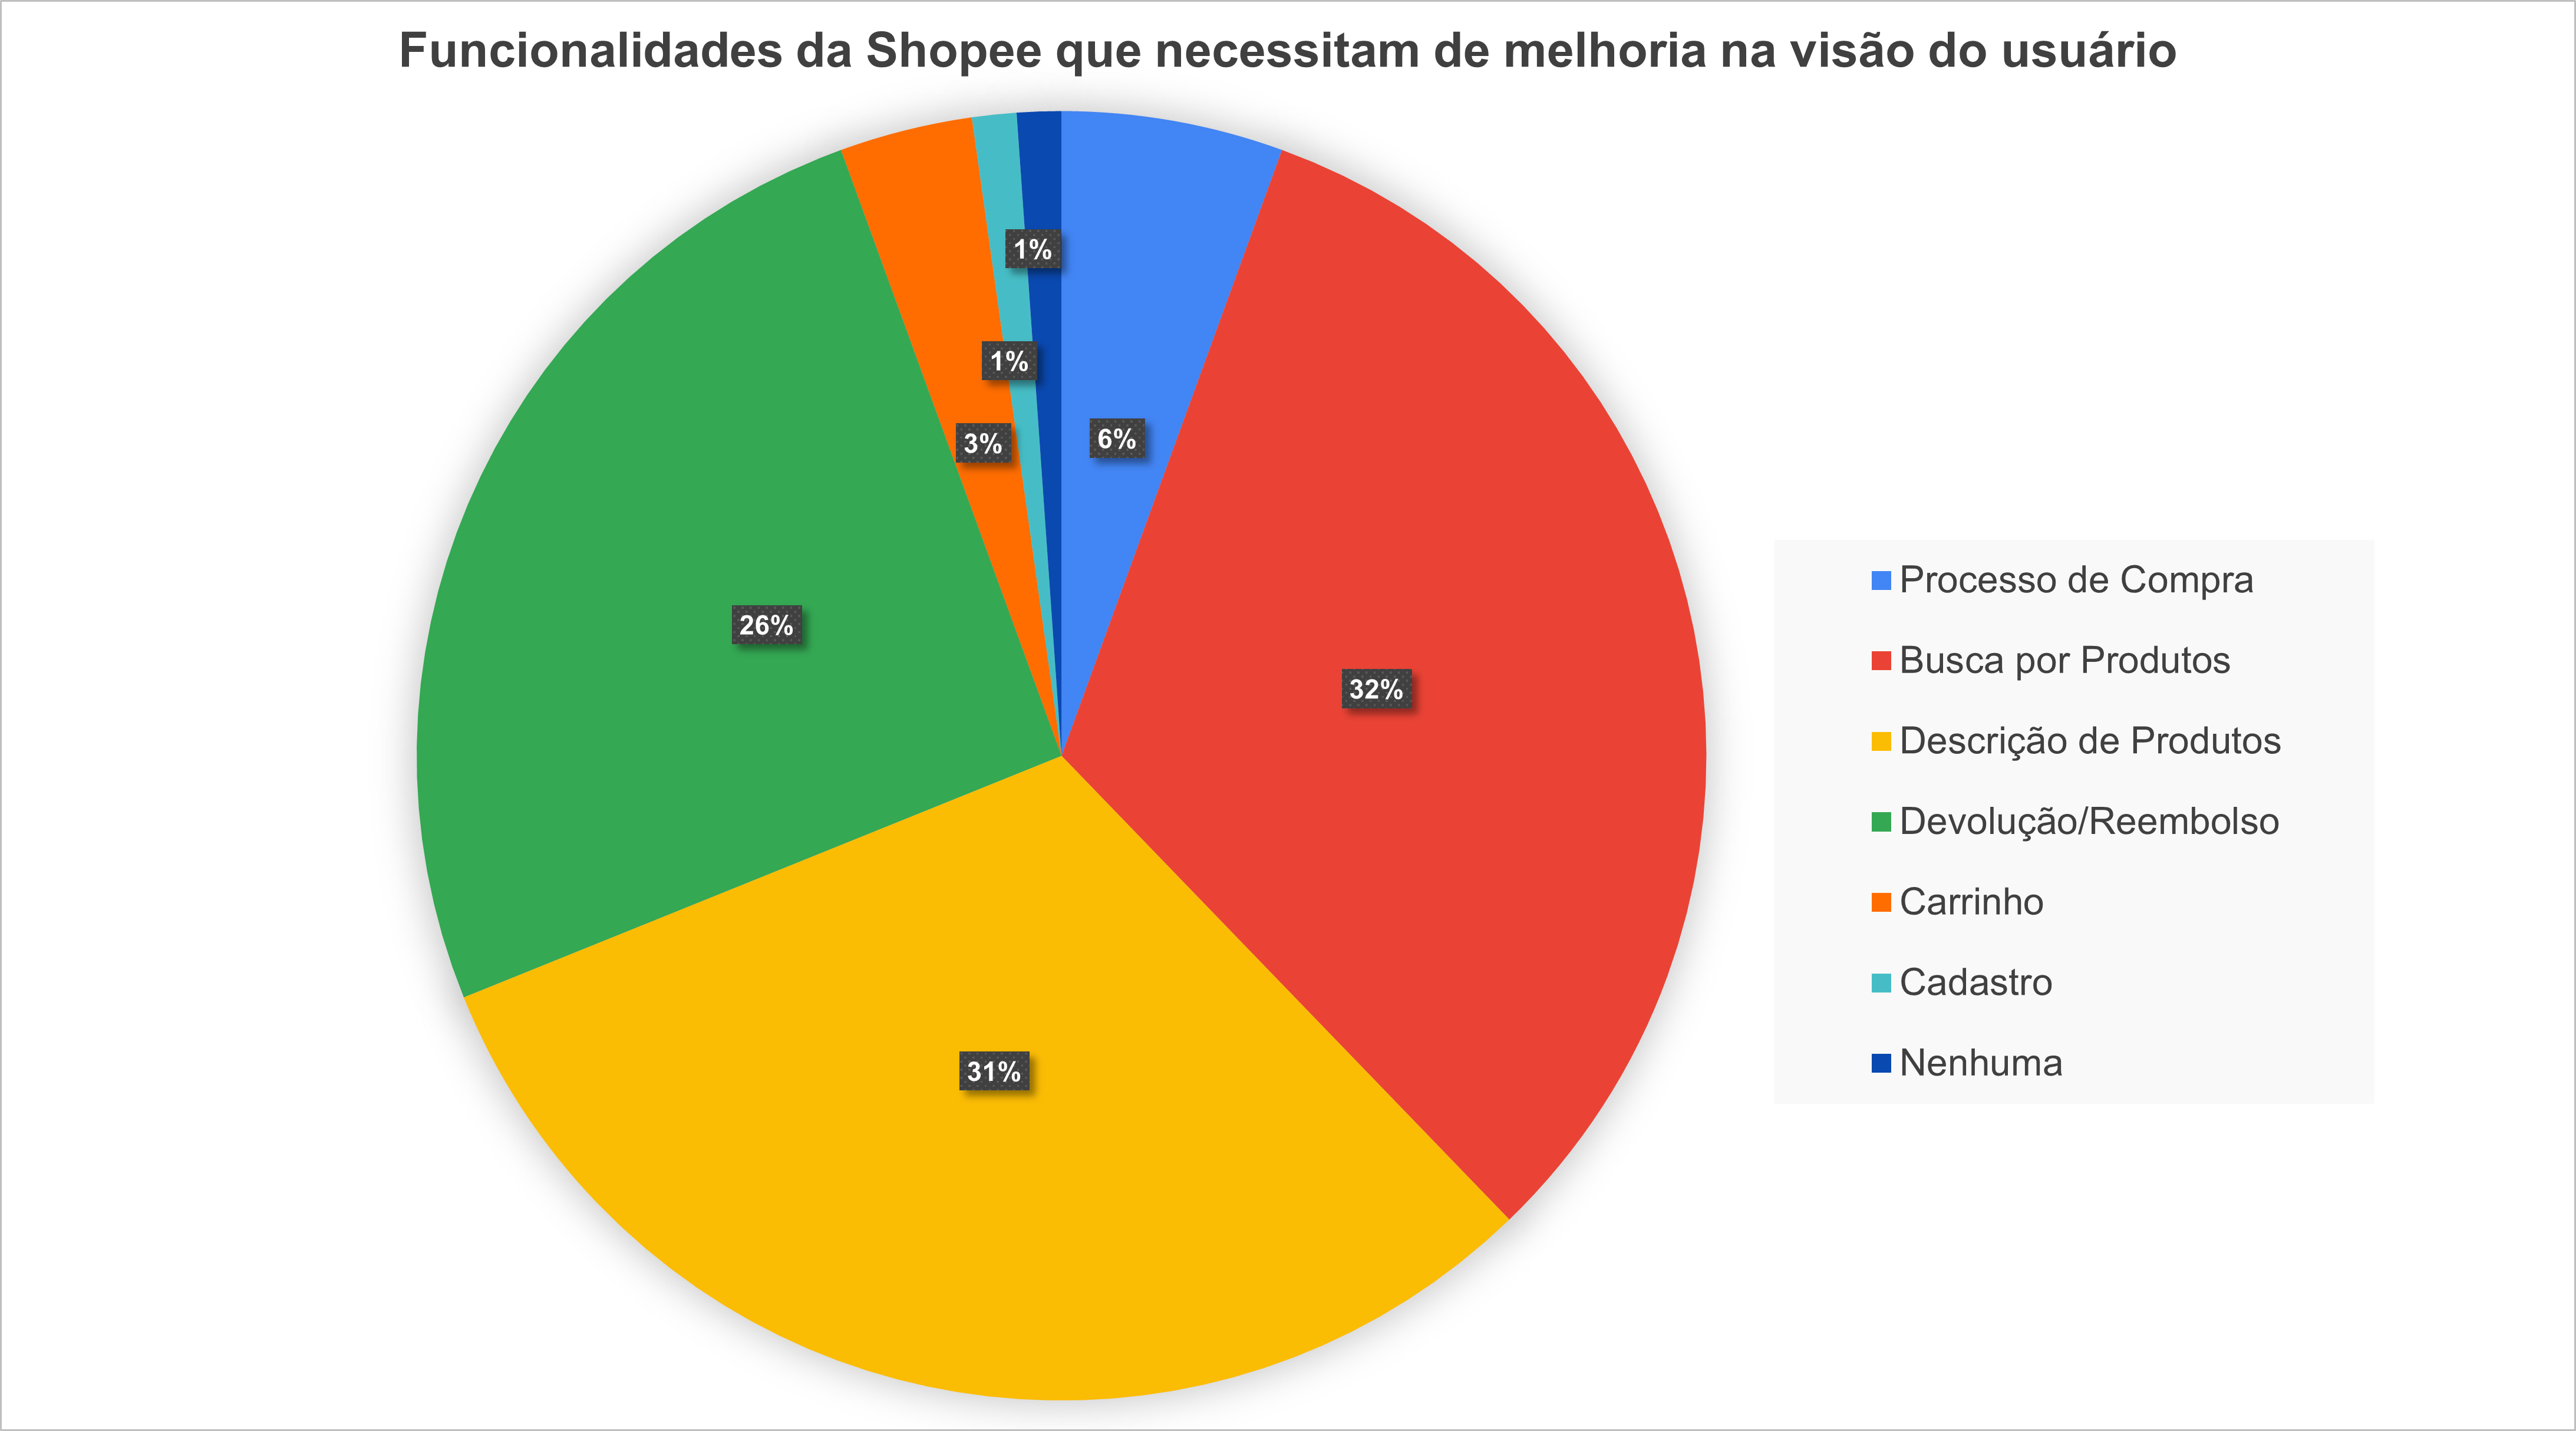
\includegraphics[keepaspectratio=true,scale=0.4]{figuras/Media_Funcionalidades_Shopee.png}
    \legend{Fonte: Autora}
    \label{FuncionalidadeShopee}
\end{figure}

Sobre a análise de métricas do AttrakDiff-R, tendo como base a Shopee, os participantes opinaram usando um sistema de pontual de sete pontos. Por exemplo, quando perguntado se o usuário considerava a aplicação Complicada ou Simples, o sistema de pontuação seria entre 1 e 3 para respostas mais próximas de Complicada, a nota 4 sendo um ponto de neutralidade entre as duas opções, e pontos de 5 a 7 mais próximas de Simples.

Tendo isso em mente, a figura \ref{MediaAtrrakShopee} exibe a média de pontos obtidos pela aplicação Shopee em cada característica abordada. Chama atenção nos resultados que nenhuma características alcançou a pontuação máxima, tendo suas maiores média em relação ao sistema ser considerado Chamativo, o que percebe-se de fato acurado já que a aplicação usa bastante de fatores visuais para mostrar promoções, ofertas, cupons e utiliza de gamificação para manter o usuário conectado. Também teve média alta a característica "Bom", sendo a Shopee sendo considerada uma aplicação satisfatória ao olhos do usuário.

Na figura \ref{MediaAtrrakShopee}, as características com menor pontuação foram "Confuso - Bem Estruturado" o que é algo preocupante para aplicação, os usuários consideraram o sistema confuso em alguns aspectos, o que é possível entender diante da analise de fluxos realizada no tópico anterior a esta seção.

\begin{figure}[ht]
    \centering
    \caption{Média AttrakDiff-R da Shopee}
    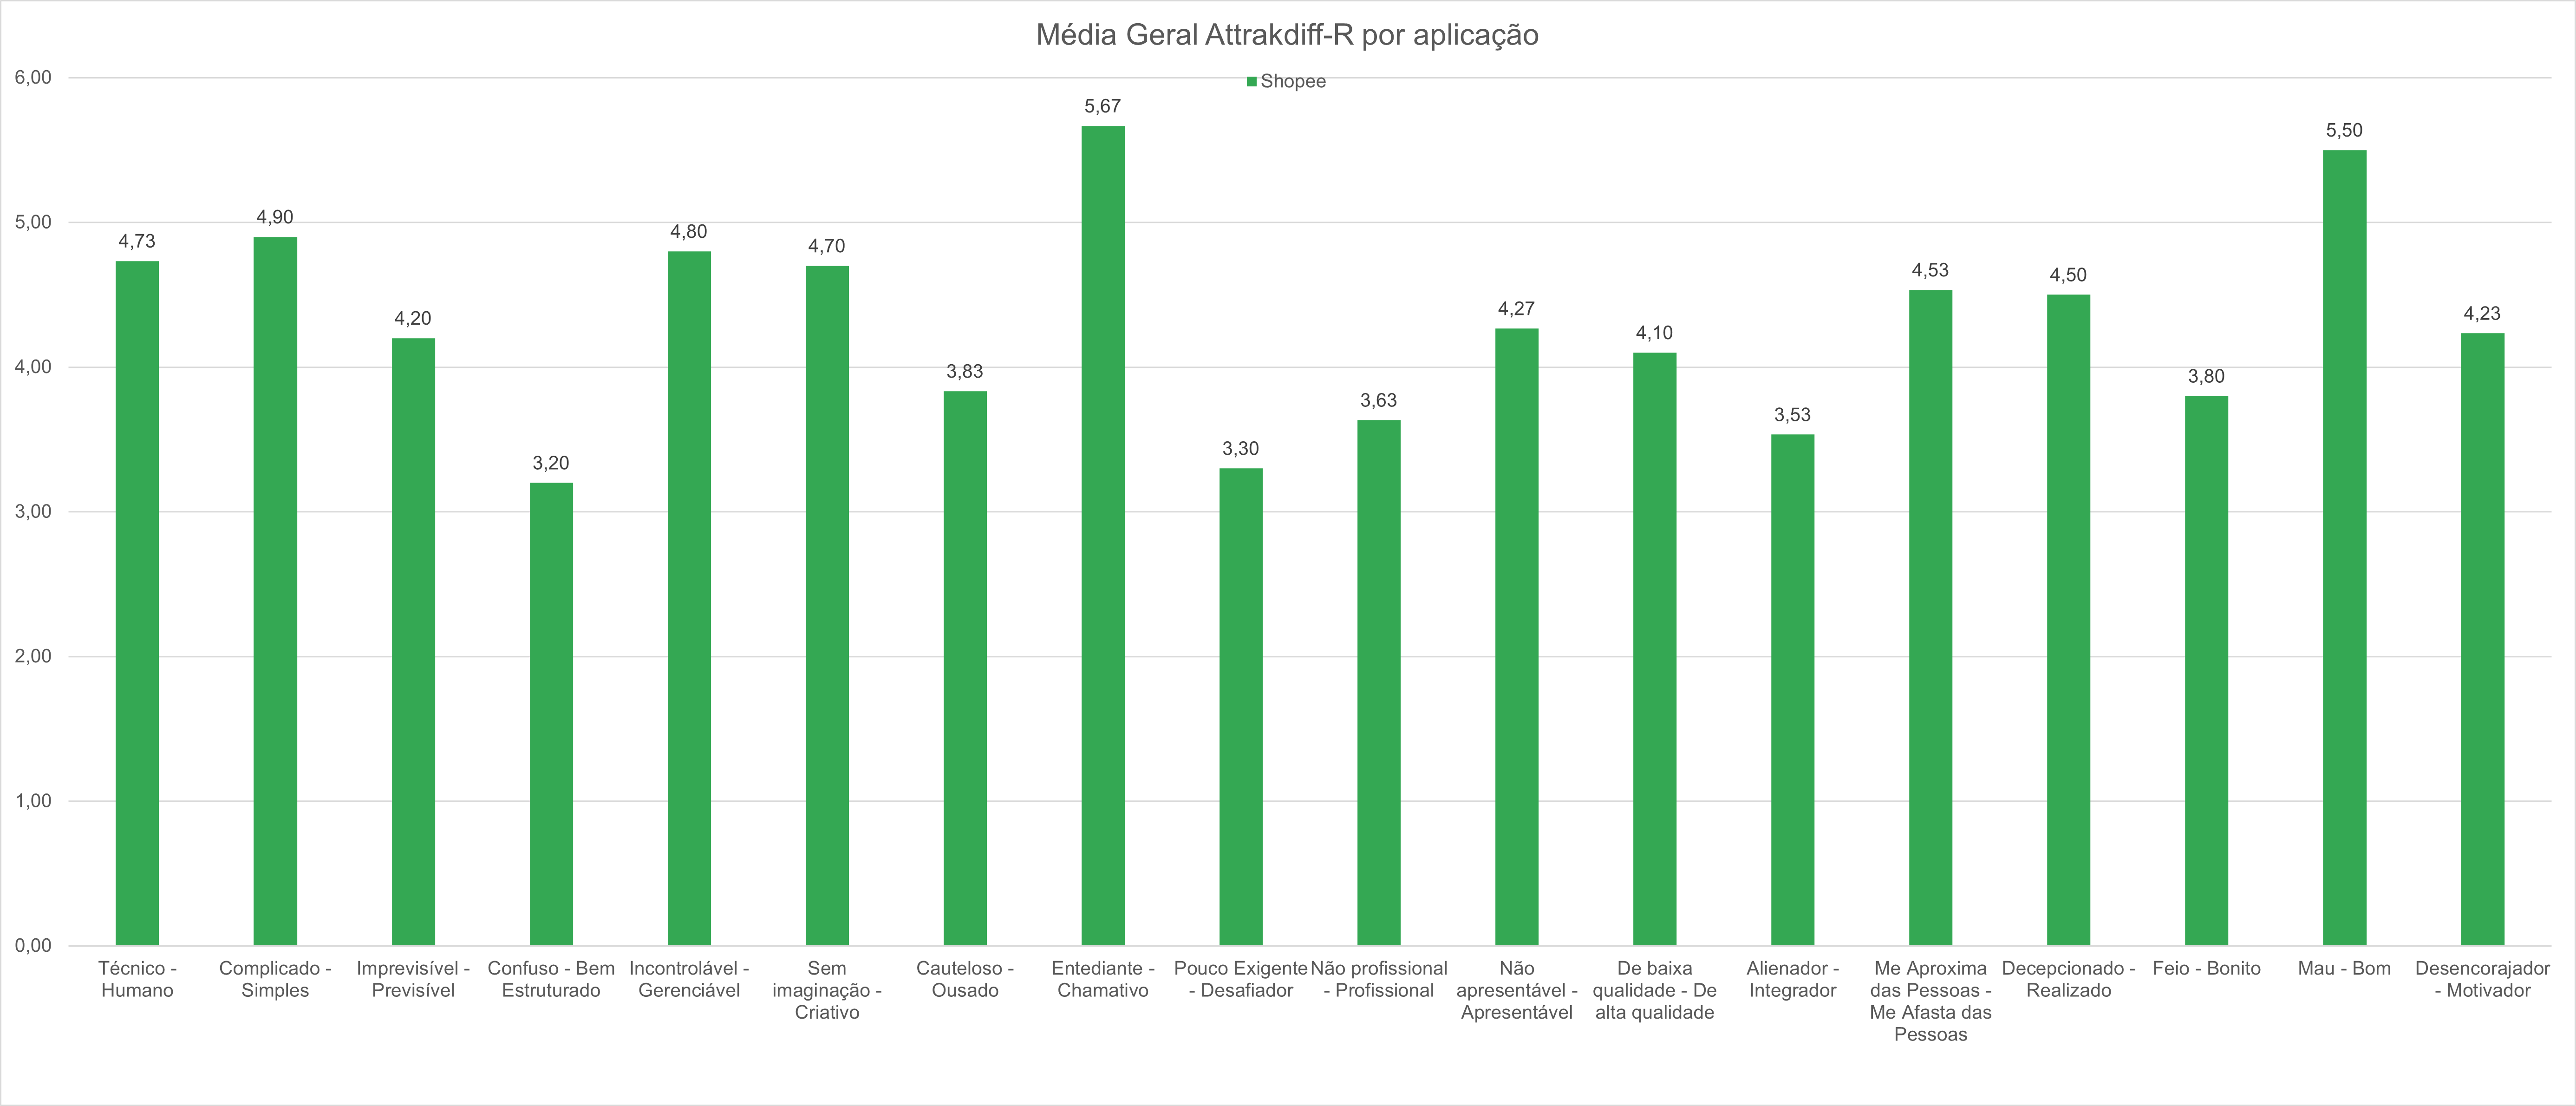
\includegraphics[keepaspectratio=true,scale=0.3]{figuras/Media_Aplicacao_Shopee_eixoY.png}
    \legend{Fonte: Autora}
    \label{MediaAtrrakShopee}
\end{figure}

Por fim, analisando as dimensões propostas pelo AttrakDiff-R, a figura \ref{ShopeeDimencoes} mostra a média obtida em cada uma pela aplicação Shopee. Percebe-se que todas as dimensões tiveram suas médias neutras, o que significa que a aplicação é um pouco ambígua para os usuários pois assim como alguns tiveram facilidades no uso outros apresentaram outro cenário. Um dos princípios das Heurísticas de Interface Móveis citada por \citeonline{HeuristicasResumo}, é que o sistema seja universal e não focado em apenas um tipo de experiência, mostrando que a aplicação pode melhorar utilizada boas práticas de usabilidade.

Quanto a dimensão Qualidade Pragmática (QP), que analisa o desempenho geral da aplicação, obteve média 4,48 mostra que, apesar dos usuários conseguirem alcançar seus objetivos, há oportunidade para a aplicação de muitas melhorias, sendo o sistema considerado Simples para o que se propõe, porém Confuso ao utilizá-lo. Já sobre a Qualidade Hedônica-Estímulo (QH-E) e a Qualidade Hedônica-Identidade (QH-I), que analisa a evolução do usuário e se identificam com a aplicação, obteve média 4,34 e 4,07 respectivamente, é perceptível que o usuário no geral tem uma relação de conexão com a aplicação neutra, o que fica evidente nos fluxos que priorizam a quantidade de vendas, em detrimento de outros aspectos relevantes. Nesses fluxo, há repetição de botões, anúncios incompletos ou incorretos, entre outros. Por fim, a Atratividade (AT), que analisa a percepção global da aplicação, obteve média 4,57 mostra um resultado neutro, porém com alto índice de considerado bom pelos usuários o que se justifica pela popularidade da aplicação ao redor do mundo.

\begin{figure}[ht]
    \centering
    \caption{Média AttrakDiff-R da Shopee por Dimensões}
    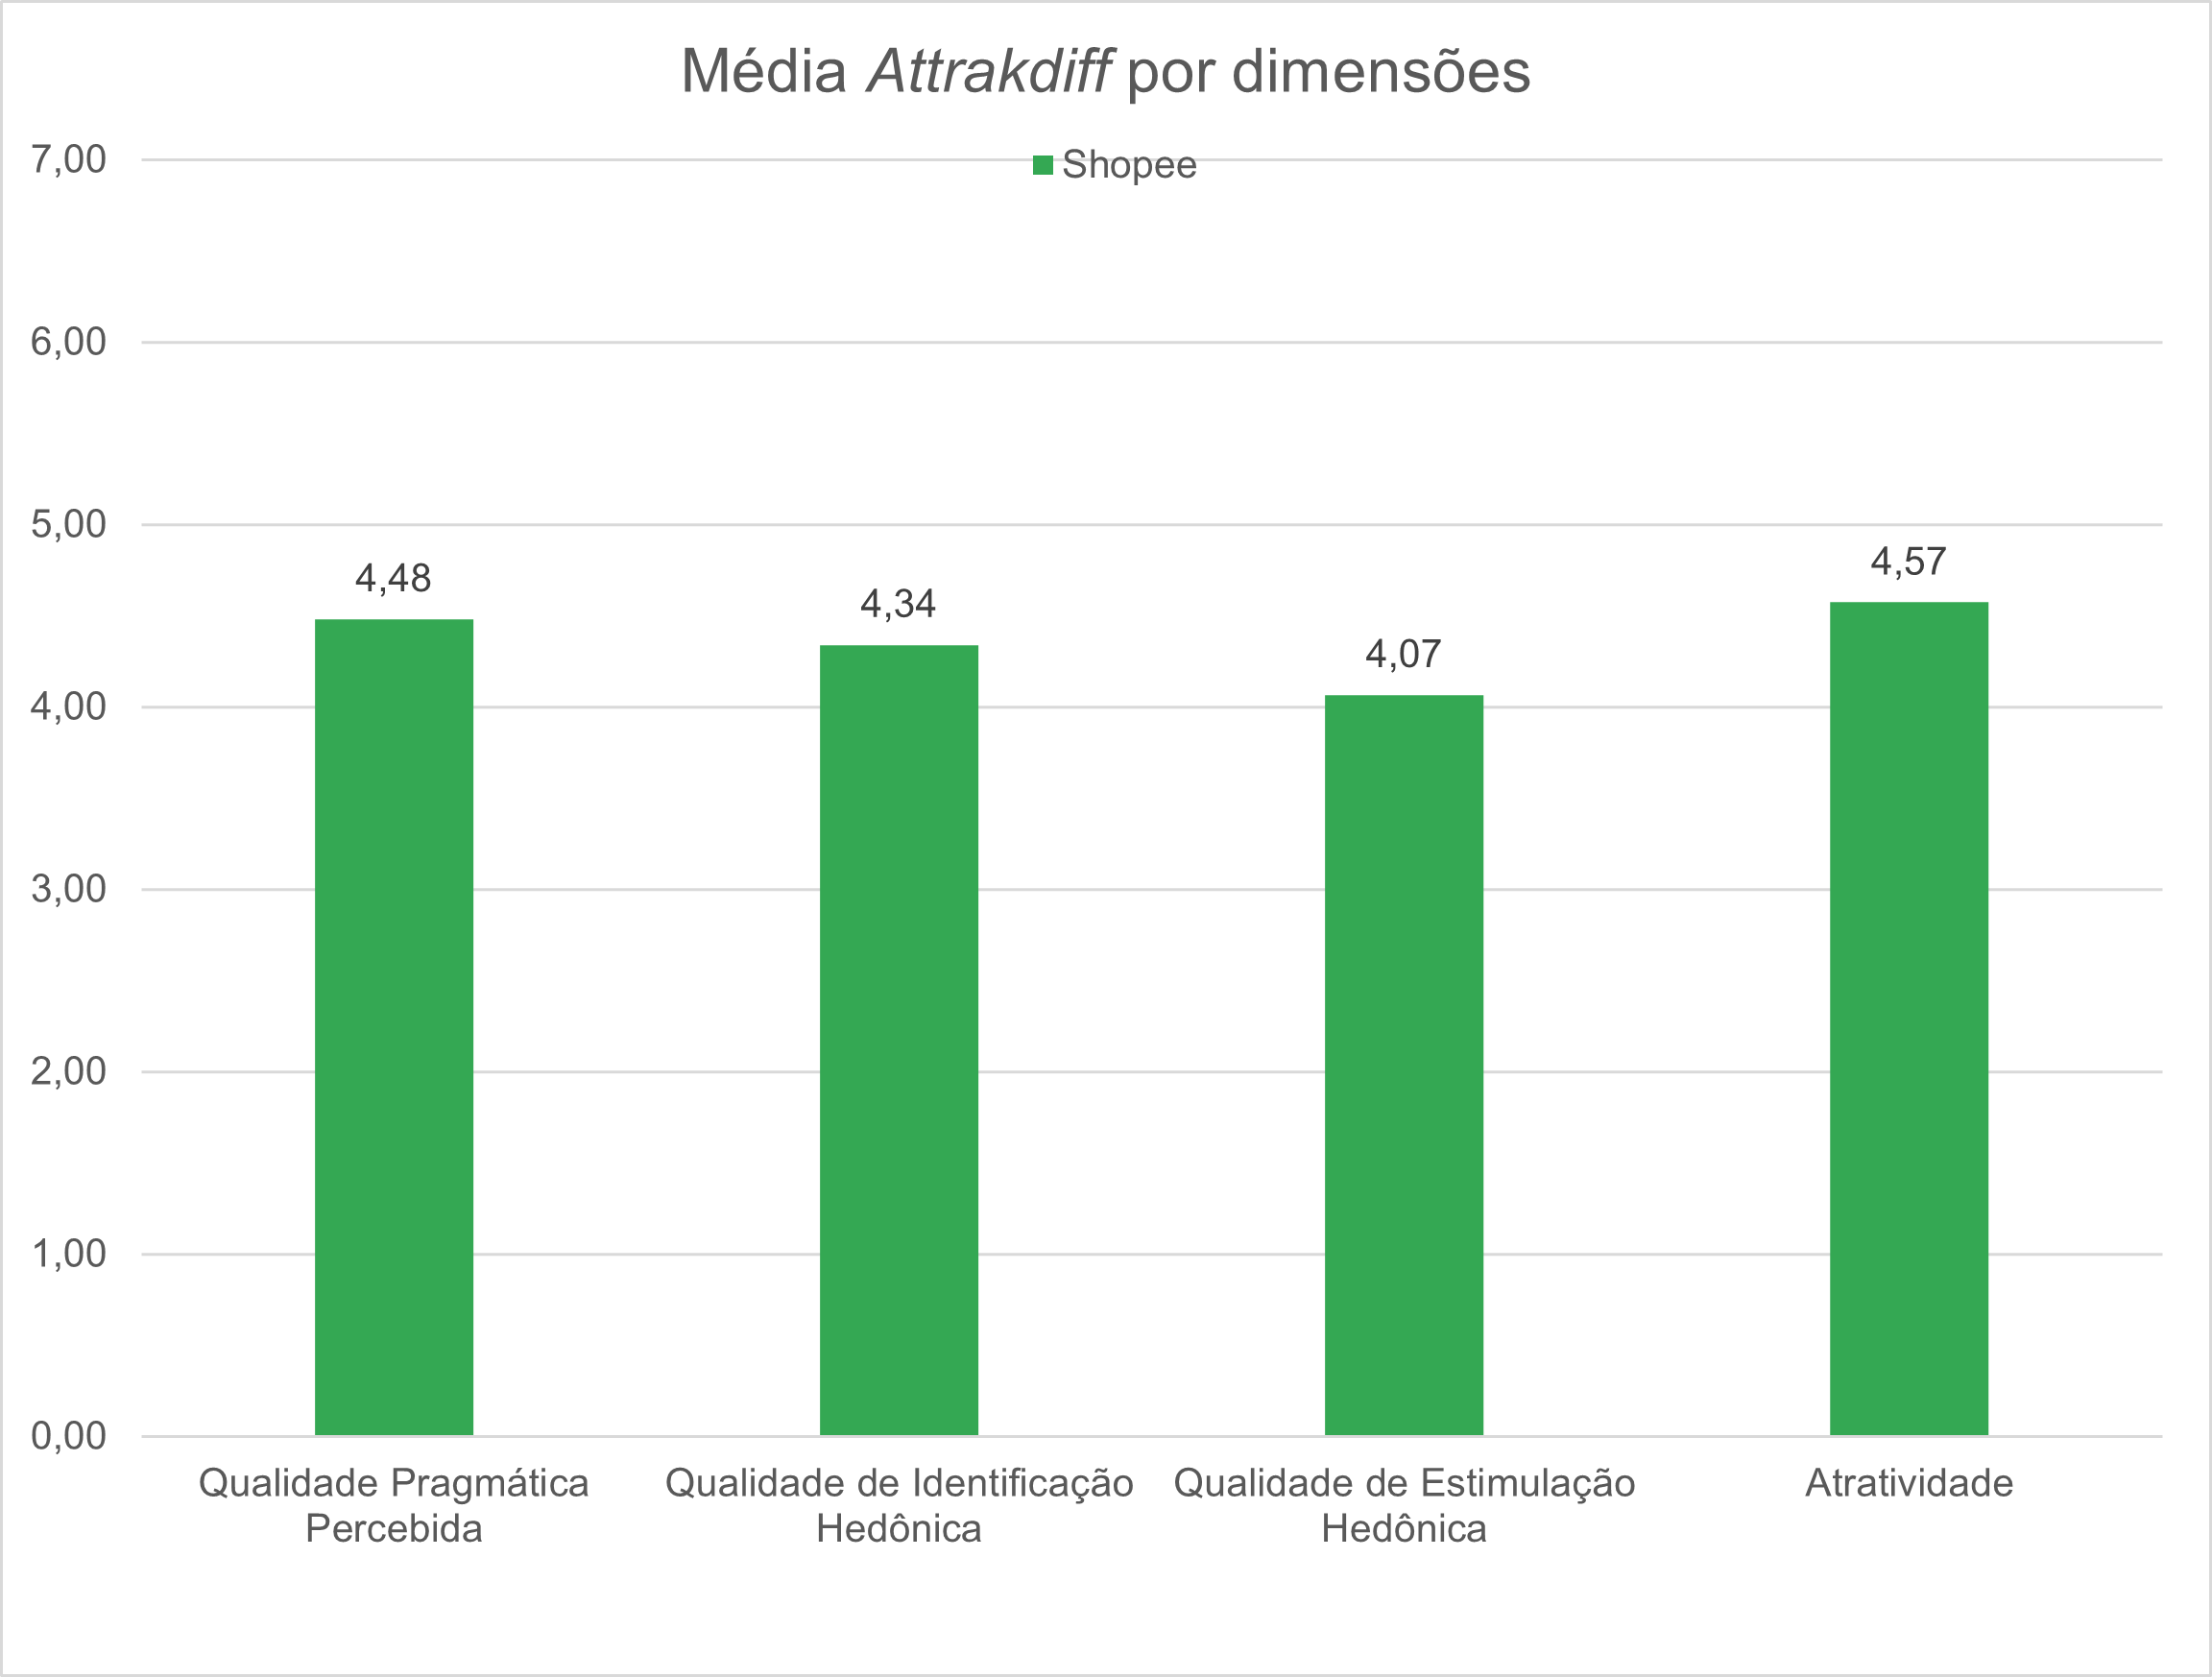
\includegraphics[keepaspectratio=true,scale=0.6]{figuras/Media_Attrakdiff_dim_7_shopee.png}
    \legend{Fonte: Autora}
    \label{ShopeeDimencoes}
\end{figure}


\section{Resumo do Capítulo}
    \label{ResumoProposta}

O capítulo abordou questões relacionadas à proposta deste trabalho, começando pela Contextualização que relembrou aspectos importantes da pesquisa e objetivos do trabalho. Sendo assim, ocorreu a apresentação da aplicação Shopee. Essa foi escolhida como a aplicação para condução do estudo exploratório, no domínio de Comércio Eletrônico Móvel, mais precisamente em âmbito nacional, Brasil. Para esclarecer sobre alguns pontos de relevância da proposta, foi acordada uma Prova de Conceito. Nesse caso, foi detalhada sobre a aplicação Shopee, levantando insumos sobre sua popularidade, bem como sobre seus principais fluxos e funcionalidades oferecidos aos usuários. Destacou-se ainda sobre pontos candidatos à melhoria, com foco na Usabilidade orientada pela Experiência de Usuário, apresentando telas que ilustram as dificuldades encontradas pelos usuários ao interagirem com a plataforma online. Por fim, foi conduzida uma análise de resultados preliminar, usando como base o questionário AttrakDiff-R. Como conclusão, reforça-se a premissa de que há abertura para melhorias na aplicação Shopee, no tange Usabilidade orientada à Experiência de Usuário.


